\chapter{Определение смысловой близости пары ключевых слов} \label{chapt1}
В настоящем разделе подробно описываются алгоритмы определения семантической близости пары ключевых слов. Разработанные модели определения семантической близости является важным результатом деятельност в рамках настоящей диссертации.
Для определения близости вводятся вспомогательные графы, вершинами которых являются ключевые слова, а ребра указывают на некоторые свойства пары ключевых слов.
На основе построенных графов с помощью методов из теории графов вычисляются различные количественные характеристики, необходимые для выявления семантической связи между рассматриваемыми словами.
После этого предлагаются способы применения методов машинного обучения, которые в значительной мере улучшают качество определения смысловой близости между ключевыми словами. 
Также описывается новый алгоритм автоматического формирования обучающей выборки для машинного обучения. Важность данного алгоритма в том, что он избавляет от необходимости ручной разметки данных, которая обычно является трудозатратной работой.
В конце раздела представлены результаты тестовых испытаний программных реализаций алгоритмов, выводы о выполненной работе, а также предлагаются идеи для дальнейшего улучшения качества определения семантической близости наборов ключевых слов.

\section{Графовые алгоритмы выявления семантической информации}
Дано множество документов $D$ и множество ключевых слов $W$. Каждый элемент $d_i \in D$ представлен набором из $k_i$ ключевых слов из множества $W: d_i = (w_{i,1},w_{i,2},...,w_{i,ki})$. Необходимо разработать такую функцию близости $WordSim : W \times W \rightarrow [0, 1]$, высокие значения которой означали бы высокий уровень смысловой близости между ключевыми словами. В следующих далее разделах описываются необходимые вспомогательные алгоритмы, модель определения семантической близости и тестовые испытания реализации этой модели.

\subsection{Построение графа близости ключевых слов} \label{sect1_1}
Вычисление смысловой близости пары ключевых слов основывается на построении графа ключевых слов. Вершины этого графа соответствуют ключевым словам, а взвешенные ребра отражают факт вхождения слов в один набор. Значение веса ребра между вершинами $i, j$ графа $G$ определяется формулой:
$$ G(i, j) = \sum_{\{T|i\in T, j \in T\}}\frac{1}{|T|}, $$
где суммирование проводится по всем наборам $T$, которые содержат в себе оба слова $i$ и $j$.

Таким образом, если слова часто встречаются в  коротких наборах, то вес соответствующего ребра в графе будет высоким. Эта характеристика является важной для определения семантической близости, но не определяющей: слова не обязаны быть похожими друг на друга по смыслу. Напротив, нередко они служат для того, чтобы более точно описать общую тему документа, к которому относятся, а добавление точного синонима не добавляет информации о тематике документа. 

Следует однако отметить, что в таком виде граф не дает значительного улучшения результата. Это происходит вследствие того, что ребра между непохожими друг на друга вершинами <<зашумляют>> значения формул:   высокое значение формулы начинает больше указывать на уровень употребимости пары слов вместе, чем на семантическую близость между ними. Чтобы избежать подобного эффекта, была разработана более эффективная модель вычисления контекстной близости для пары ключевых слов, описанию которой посвящен следующий далее раздел.


\subsection{Модель определения контекстной близости для пары ключевых слов} \label{cont_sim}
Важной идеей новой модели вычисления смысловой близости по сравнению с моделью, описанной ранее в главе [???] является следующее наблюдение: уровень похожести слов x и y увеличивается, если существует большое число слов $k$, входящих в одни наборы и с $x$, и с $y$. С учетом этого факта была разработана модель определения контекстной близости, описание которой приводится далее. Согласно проведенным тестовым испытаниям, контекстная близость является более точной аппроксимацией смысловой близости, чем близость, введенная ранее в [???]. Общие слова $k$ в рамках новой модели выступают в роли общего контекста для слов $x$ и $y$. Вычисления контекстной близости для пары вершин производится по графу ключевых слов. При этом высокие частоты вхождений слов $x$ и $y$ в различные наборы негативно влияют на уровень близости: частотные слова склонны иметь больше общих контекстов. Таким образом возникает естественная идея нормировки близости на частоты встречаемости слов, для которых необходимо вычислить уровень близости. 

Кроме того, поскольку слова $x$, $y$ и $k$ могут все входить в один набор, то в таком случае связь слов $x$ и $y$ через слово $k$ будет отражать скорее факт совместной встречаемости $x$ и $y$ в одном наборе, а не контекстную близость этой пары слов. Cовместная встречаемость далеко не всегда влечет сильный уровень семантической близости. Характер этой связи частотности и смысловой схожести во многом зависит от сферы, в которой применяются ключевые слова, и от того, с какой целью пользователи системы эти ключевые используют. Например, ключевые слова для научной публикации редко содержат в себе синонимы, поскольку эти слова используются для того, чтобы дать читателю понять о чем будет статья. Точные синонимы для слов в этом случае не несут никакой дополнительной информации о данной области. Вследствие этого, высокая частота совместной встречаемости не ведет к семантической близости и должна пессимизировать значение формулы контекстной близости. Другим примером являются ключевые слова в социальных сетях. Пользователи используют ключевые слова к документам таким образом, чтобы этот документ было легче найти среди других документов системы. Поэтому, использование синонимов, переводов, транслитерации, различных способов написания ключевых слов помогает в поиске документа. При этом, однако, не добавляет никакой смысловой информации непосредственно к описанию этого документа. Примеры различных наборов ключевых слов из разных областей будут даны в разделе <<Тестовые испытания>>. Исходя из этих соображений, предлагается две представленные далее формулы для вычисления контекстной близости для пары ключевых слов.

Для пары ключевых слов $i$, $j$ контекстная близость определяется по формулам:

\begin{equation}
    \begin{aligned}
       C_{\+}(i, j) = \frac{C(i, j) * \log(1 + m(i,j))}{f(i) + f(j)},\\
       C_{\-}(i, j) = \frac{C(i, j)}{(1 + m(i,j)) * f(i) + f(j)},
    \end{aligned}
\label{eq:test}
\end{equation}
где $C(i,j)$ - контекстная близость между $i$ и $j$ внутри графа, $m(i,j)$- частота совместной встречаемости в наборах пары $i$, $j$, $f(i)$- индивидуальная частота встречаемости слова $i$ в наборах. В программной реализации алгоритмов частоты $f(i)$ и $m(i,j)$ для удобства сохраняются при построении графа ключевых слов в качестве дополнительной информации, соответственно, в вершинах и в ребрах графа.

\subsection{Построение полного контекстного графа ключевых слов}
Вершинами контекстного графа, как и в случае графа, описанного ранее в разделе \ref{sect1_1}, являются ключевые слова. Ребро в таком графе свидетельствует о том, что пара ключевых слов является контекстно близкой. Для того, чтобы определить, соединены ли два ключевых слова ребром, необходимо посчитать контекстную близость по формулам, описанным в предыдущем разделе. В общем случае, для определения всех связей потребовалось бы $O(n^2)$ действий, где $n$- число вершин. Однако с помощью представленного далее алгоритма, это задача может быть решена за $O(nm^2)$ действий, где $m$- максимальное число соседей у вершины в графе ключевых слов.

\begin{enumerate}
    \item Построение графа ключевых слов $G$ по входным наборам ключевых слов $D$
    \item Подсчет частот встречаемости $f(i)$ и $m(p, q)$ для каждого слова $i$ и каждой пары $(p, q)$ по входным наборам из $D$
    \item Инициализация разреженной матрицы $C$ размером $n * n$
    \item Для каждой вершины $i$ графа ключевых слов:
        \begin{enumerate}
            \item Для каждой пары соседей $(p, q)$ вершины $i$:
                \begin{enumerate}
                    \item $C(p, q) \mathrel{{+}{=}} min(G(p,i), G(q,i))$
                \end{enumerate}
        \end{enumerate}
    \item Для каждой ненулевой пары $(i, j)$ матрицы $С$:
        \begin{enumerate}
            \item $C_{\+}(i, j) = \frac{C(i, j) * \log(1 + m(i,j))}{f(i) + f(j)}$
            \item $C_{\-}(i, j) = \frac{C(i, j)}{(1 + m(i,j)) * f(i) + f(j)}$
        \end{enumerate}
\end{enumerate}

\textbf{Утверждение 1.} Расчет весов $C_{+}(i, j)$ и $C_{-}(i, j)$ по построенному графу ключевых слов имеет сложность $O(nm^2)$, где $n$ - число вершин графа ключевых слов, $m$ - максимальное число ребер у вершины в графе ключевых слов.

\textbf{Доказательство.} Поскольку индивидуальные и парные частоты $f(i)$ и $m(i,j)$  уже были рассчитаны при построении графа ключевых слов, их получение имеет сложность $O(1)$.  Остается лишь вычислить сложность подсчета формул $C(p,q)$. Для вычисления требуется пройтись по всемn вершинам графа и для каждой вершины рассмотреть все пары ее соседей. Поскольку у вершины не более $m$ соседей, то обработка одной вершины занимает $O(m^2)$, а всех вершин, соответственно, $O(nm^2)$. Таким образом, и общее время работы алгоритма составляет $O(nm^2)$, что и требовалось доказать.

В целях большей оптимизации времени на построение контекстного графа разумным является ограничения числа рассматриваемых соседей для текущей вершины $i$. Данная оптимизация выполняется следующей модификацией п.4 описанного ранее алгоритма:

\begin{enumerate}
  \setcounter{enumi}{4}
  \item Для каждой вершины $i$ графа ключевых слов:
      \begin{enumerate}
          \item Сортировка соседей вершины $i$ по убыванию весов в ребрах
          \item Выделение множества $N_(i)$- первых $k$ соседей из сортированного в п.4.a списка соседей для вершины $i$
          \item Для каждой пары соседей $(p,q)$ из множества $N_k(i)$ вершины $i$:
              $$ C(p, q) \mathrel{{+}{=}} min(G(p,i), G(q,i)) $$
      \end{enumerate}
\end{enumerate}

В данном случае появляется дополнительный параметр модели $k$ (обычно в диапазоне от 10 до 30), который подбирается исходя из природы коллекции данных, а также по вычислительной производительности машины, на которой запущены расчеты. Отмечается, что предварительная сортировки соседей вершины $i$ по весам ребер позволяет использовать наиболее важных соседей в первую очередь. В результате этого на практике появляется способ значительно уменьшить количество вычислений и при этом построить модель, не уступающую в качестве модели, в которой рассматривается полный набор соседей для вершины. В некоторых случаях удаление менее значимых вершин дает даже прирост в качестве, поскольку зачастую такие вершины являются шумовыми для определения семантической близости.

Построение контекстного графа, в котором для вершины рассматриваются не все ее соседи, имеет вычислительную сложность $O(nk^2+m\log(m))$, что показано в следующем утверждении.

\textbf{Утверждение 2.} Расчет весов $C_{+}(i, j)$ и $C_{-}(i, j)$ по построенному графу ключевых слов для случая ограниченного числа рассматриваемых соседей для текущей вершины имеет сложность $O(nk^2+m\log(m))$, где $n$ - число вершин графа ключевых слов, $k$ - количество рассматриваемых соседей.

\textbf{Доказательство.} Аналогично предыдущему утверждению, за исключением того, что теперь для текущей вершины будет рассмотрено порядка $O(k^2)$ пар соседей. Кроме того появляются дополнительные затраты на сортировку соседей вершины (п.4.а последнего алгоритма), которые занимают $O(m\log(m))$ времени. 

При $k=\sqrt{m}$, например, достигается оценка $O(nm)$ времени работы, что является значительным ускорением работы алгоритма.

Таким образом, данный алгоритм позволяет за время, относительно небольшое по сравнению с наивным перебором всех пар вершин, расчитать контекстный граф, собранный по данным из миллионов наборов ключевых слов, поскольку в среднем каждое слово соединено с небольшим числом других слов. Следует также отметить, что отношение контекстной близости коммутативно, поэтому хранить достаточно только верхний правый угол матрицы $C(p,q)$.

\subsection{Построение усеченного контекстного графа ключевых слов}
Обозначим теперь за $C_{*}(i,j)$ любую из формул $C_{+}(i,j)$ или $C_{-}(i,j)$. Ненулевое значение $C_{*}(i,j)$ означает контекстную связь между ключевыми словами. Несмотря на то, что такие матрицы контекстной близости остаются сильно разреженными, существует огромной число ненулевых связей, что делает затруднительным их дальнейший анализ с технической точки зрения. В дополнении к этому, низкие значения близости могут являться шумом. Такие данные не привносят полезной информации, а только ухудшают качество алгоритмов. По этим причинам возникает практическая необходимость в усечении графа, собранного описанным выше алгоритмом. Под усечением понимается удаление ребер, которые представляют наименее качественные и статистически проверенные связи. 

По результатам экспериментов на коллекциях данных, описанных далее в разделе <<Тестовые испытания>>, была установлена следующая стратегия отбора важных связей для данной вершины $i$:
\begin{enumerate}
    \item \textbf{Для всех $j$ удаляются связи со слишком низким уровнем близости $C_{*}(i,j)$.}

    Этот шаг необходим для того, чтобы удалить <<шумные>> и слабые связи из рассмотрения. Стоит также отметить, что по результатам экспериментов было проверено, что одного этого правила недостаточно для качественного обрезания лишних ребер. Причиной этому является тот факт, что сами значения близости $C(i,j)$ не так важны, как порядок, который они задают на множестве соседей вершины $i$.  Другими словами, данная задачу фильтрации стоит рассматривать как задачу ранжирования соседей вершины $i$ , а не как задачу классификации пар $(i, j)$ на классы полезных и бесполезные ребер.
    \item \textbf{От оставшихся выбирается некоторая доля связей (например, 20\%) с наибольшими значениями $C_{*}(i,j)$ .}

    Это условие видится естественным, потому что слова, которые встречаются со многими другими в одинаковых контекстах, должны иметь больше ребер в графе, чем те слова, которые контекстно близки только с небольшим числом слов.

    \item \textbf{Количество отобранных связей должно находиться в некоторых рамках (например, не менее 3 и не более 10 соседей на вершину).}

    Верхняя граница является преимущественно техническим ограничением: если было взято 20\% от числа всех соседей, но это число по-прежнему достаточно велико, то хранение таких вершин потребует значительных ресурсов. Нижняя граница берется для того, чтобы вершина, для которой имеется мало кандидатов, получила хотя бы их в качестве ребер. С учетом ограничения из п.1. можно ожидать, что эти связи будут достаточно качественными для дальнейшего анализа.
\end{enumerate}

Следует также отметить, что окончательное число соседей для данной вершины $i$ может быть несколько больше, поскольку лишние связи могли породиться одним из соседей вершины в полном графе, это означает, что ребро $(i,j)$ может существовать, потому что оно прошло фильтрацию ребер для вершины $j$, а не для вершины $i$. Далее приведено более формальное описание алгоритма, реализующего введенную выше модель.

\begin{enumerate}
    \item Все значения близости, меньшие порогового  t, приравниваются нулю:

        $$C_{*}(i,j):=0, если C_{*}(i,j) < t. $$
    \item Пусть $rank_j$- порядковый номер соседа $j$ в отстортированном по убыванию значения $C_{*}(i,j)$ списке всех соседей вершины $i$. Тогда, если $rank_j >\max(n_{min},min(n_{max},n * r))$, то связь $(i,j)$ должна быть отфильтрована. Здесь $n_{min},n_{max}$ - минимальное и максимально число ребер для одной вершин в новом графе. $n$- число соседей вершины в полном контекстном графе, $r$- доля ребер, которую необходимо перенести в усеченный граф.
\end{enumerate}

Среди описанных выше параметров только параметр $t$ требует анализа для подбора. Остальные пороговые значения легко могут быть выбраны, исходя из специфики задачи. Подбирать t можно эмпирически или по небольшой размеченной выборке примеров контекстно похожих слов. Отмечается, что tдолжен быть выбран так, чтобы полнота выбранных ребер оставалась достаточно высокой.

Отмечается также, что ребра построенного графа могут быть помечены числами, ввести функцию расстояния между вершинами. Например, такой функцией может служить величина $C_{*}(i,j)$. В рамках рассматриваемого подхода, ребра графа остаются непомеченными, что существенно понижает сложность разработанных моделей.

\subsection{Процедура кластеризации усеченного контекстного графа}
Ребра усеченного контекстного графа, который был введен в предыдущем разделе, в большей мере показывают семантическую близость между парой вершин, чем ребра полного контекстного графа или, тем более, графа ключевых слов. Помимо того, что усеченный граф значительно уменьшает вычислительные затраты, он повышает точность выявленных семантических связей между ключевыми словами, жертвуя при этом полнотой. В этой связи рассмотрение длинных путей в графе становится более оправданным, поскольку семантическая близость между парой вершин лучше сохраняется с увеличением расстояния в графе. Вследствии этого возникает задача кластеризации графа: разделение множества всех вершин на подмножества таким образом, что любая пара вершин из одного множества является парой близких по смыслу ключевых слов. 

За основу кластеризующего алгоритма взят алгоритм Louvain Modularity \cite{louvain_modularity}. В ходе работы алгоритма максимизируется значение функционала модульности: 

$$ Q = \frac{1}{2m}\sum_{i,j}[A_{ij} - \frac{k_i k_j}{2m}]\delta(c_i, c_j) $$

где $\delta$- дельта функция, $A_{ij}$- вес ребра между вершинами $i$ и $j$, $k_i=\sum_j{A_{ij}}, m=\frac{1}{2}\sum_{i,j}A_{ij}$. Как показано авторами \cite{modularity_is_hard}, задача максимизации выписанного выше функционала является NP-сложной, поэтому для её  решения используются аппроксимационный алгоритм, основные шаги которого описаны далее.

\begin{enumerate}
\item Для каждой вершины графа создается свой кластер.
\item Для каждой вершины $i$ и для каждого соседа $j$ вершины $i$:
    \begin{enumerate}
        \item временное добавление вершины $i$ в кластер вершины $j$;
        \item подсчет изменения оптимизируемого функционала $\Delta Q$;
        \item окончательное добавление вершины iв кластер того соседа, на котором достигается максимальное увеличение значения $Q$. Если функционал невозможно увеличить, то добавления не происходит.
    \end{enumerate}
\item Построение нового графа, вершинами которого являются кластера, а веса ребер отражают связи между кластерами. Вес ребра равен сумме весов всех пар ребер, вершины которых лежат в соответствующих кластерах.
\end{enumerate}

Преимущество данного алгоритма в его масштабируемости на графы больших размеров. Качество кластеризации при этом остается на высоком уровне. Отмечается, что количество кластеров не является параметром данного алгоритма. На практике кластера, получающиеся в результате работы программной реализации алгоритма, оказываются слишком большого размера. В некоторые кластера могут попасть тысячи или десятки тысяч слов, очевидно, что не существует такого огромного множества попарно похожих по смыслу слов. Алгоритм является общим графовым алгоритмом и никаким образом не использует информацию о семантической близости. Даже точное решение оптимизационной задачи не гарантирует качественного разбиения вершин графа на подмножества, элементы которого семантически близки друг к другу. Как следствие, необходимы дополнительные действия, связывающие процессы кластеризации графа и определения семантической близости. Далее представлена окончательная версия алгоритма кластеризации контекстного графа, разрешающая отмеченную трудность.

\begin{enumerate}
    \item Заводится очередь для подграфов исходного графа, исходный граф добавляется в нее.
    \item Пока очередь не пуста:
    \begin{enumerate}
        \item кластеризация подграфа из очереди алгоритмом Louvain Modularity;
        \item для каждого полученного в результате кластеризации подграфа-кластера:
            \begin{enumerate}
                \item если размер кластера меньше, чем $k$, то добавить кластер в выходное множество кластеров;
                \item иначе добавить кластер в очередь подграфов.
            \end{enumerate}
    \end{enumerate}
\end{enumerate}

$k$- параметр алгоритма, который выбирается из специфики задачи. Для задачи кластеризации ключевых слов значение параметра $k$ может варьироваться в пределах от 10 до 20.

% \subsection{Графовые методы выявление тематических направлений в наборах ключевых слов} %\label{sect1_2}
\subsection{Определение абстрактности слова} \label{abstract_words_chapter}
Для решения поставленной в \ref{theme_tags} задачи в следующих разделах используется понятие абстрактности ключевого слова. Под абстрактностью понимается степень общности значения слова. Необходимо разработать такую меру абстрактности $a : W \rightarrow \mathbb{R}+$, чтобы большим значениям меры соответствовали слова более широкого значения, а меньшим - слова более конкретного, обладающего определённой спецификой значения.

В настоящем разделе представлены алгоритмы определения степени абстрактности ключевых слов на основе графа ключевых слов. В наборах тегов присутствуют слова, которые
указывают на общую тематическую направленность документа, а также слова, отражающие более узкую специализацию (термины). Проиллюстрируем это на примере следующего набора ключевых слов (подчёркнуты слова более общего значения):

    \textbf{[рынок труда, профессиональная ориентация, \underline{прогнозирование}, \underline{модель}, \underline{алгоритм}]}\

Трудность решения поставленной задачи обусловлена тем обстоятельством, что необходимо уметь отделять действительно абстрактные по значению слова от слов популярных, и, как следствие, часто используемых в наборах ключевых слов.

\subsubsection{Определение степени абстрактности на основе свойства центральности}
В теории графов существует характеристика важности вершины графа, которая по-русски именуется центральность. Для того, чтобы определить влияние вершины внутри графа, существует несколько различных мер. Основные из них перечислены далее.
\begin{itemize}
    \item Центральность по посредничеству (betweenness centrality) — мера, которая определяется через количество кратчайших путей, проходящих между всеми парами вершин в графе через данную вершину. $bc(i) = \underset{s,t\in V \wedge s \neq i \wedge t \neq i}\sum_{}{\frac{n^i_{s,t}}{n_{s,t}}}$, где $n_{s,t}$ - количество кратчайших путей через вершины $s$ и $t$. $n^i_{s,t}$ - количество кратчайших путей через вершины $s$ и $t$, проходящих через $i$, $V$ — множество вершин графа;
    \item Центральность по близости (closeness centrality) - мера, основанная на средней длине кратчайшего пути между исходной вершиной и всеми другими вершинами графа.  $c_i=\frac{[\underset{j\in V_i}\sum_{}{dist(i,j)}]^{-1}}{k}$, где $dist(i,j)$ - длина кратчайшего пути между вершинами $i$ и $j$. $k$- количество вершин из компоненты связности вершины $i$. $V_i$ - множество вершин из этой компоненты связности.  \item Центральность по степени (degree centrality) - мера, в которой важность вершины равна её степени (числу инцидентных ребер);
\item Центральность собственного вектора (eigen vector centrality) - мера, описанная в \cite{eigen_vect_cent}, вычисляется по формуле $x(i) = \frac{1}{\lambda}\underset{j \in V}\sum{a(i,j)x(j)}$, где $a$ - матрица смежности графа, $\lambda$ - константа. Это выражение быть быть переписано в векторной форме следующим образом: $Ax = \lambda x$. Большее значение меры ставится той вершине, которая соединена с большим числом вершин, меры которых высоки;
\item  PageRank-центральность (PageRank centrality) - алгоритм, используемый Google для ранжирования страниц (метод определения важности или популярности документов) \cite{pagerank}.  Согласно этому алгоритму, веб-страница имеет больший вес, если на неё много ссылок из других веб-страниц, также имеющих большой вес. Заметим, что в данном виде алгоритм применим не только для веб-страниц, но и для любых графов. Общая идея этого алгоритма близка к идее, которая реализуется алгоритмом вычисления eigen vector centrality. Однако в уравнениях, которые используются алгоритмом PageRank, вместо собственных значений присутствует коэффициент затухания $q$. Физический смысл этого коэффициента в том, что пользователь имеет некоторую вероятность перехода с одной веб-страницы на другую по ссылке. При этом, он может никуда не переходить и закончить случайное блуждание по сети. Таким образом, q — это вероятность того, что пользователь перейдёт по ссылке. Получаемое уравнение имеет следующий вид: $PageRank(i) = (1 - q) + q\underset{j\in V_i}\sum{\frac{PageRank(j)}{C_j}}$, где $C_j$ - количество ссылок в документе $j$. В программной реализации параметр $q$ определен как 0.9.
\end{itemize}

Далее используется идея, что слишком длинный путь между вершинами в графе обычно не означает хотя бы какой-то связи между словами. По этой причине программная реализация алгоритмов Betweenness Centrality и Closeness Centrality сделана таким образом, чтобы длинные пути не учитывались. Для этого соответствующие меры для вершины считаются не во всем графе, а в подграфе соседей на расстоянии 3 от вершины. Для каждого из алгоритмов за меру абстрактности тега принимается мера центральности соответствующей вершины. Результаты работы программной реализации алгоритмов представлены в приложении \ref{AppendixA}. Отметим, что под степенью абстрактности следует понимать общность значения слова именно в рамках заданного корпуса слов. Это, например, означает, что слово <<вероятность>> можно считать абстрактным потому, что можно предположить, что существует много статей, посвящённых некоторым проблемам из теории вероятности. По этой причине существует много различных слов-терминов, имеющих прямое отношение к слову «вероятность».

Резюмируя представленные выше соображения, необходимо отметить, что степень абстрактности слова является достаточно субъективной величиной. По этой причине проведение объективной количественной оценки результатов работы алгоритмов на больших объёмах данных затруднительно. В качестве основного метода проверки адекватности предлагаемого метода используется выборочная экспертная оценка результатов.

\subsubsection{Окончательный алгоритм}

В качестве окончательного алгоритма авторами принят алгоритм, смешивающий
результаты представленных выше алгоритмов, а именно:

\begin{itemize}
    \item для каждого алгоритма вычисляется вектор из центральностей вершин;
    \item каждый вектор нормируется на свою сумму;
    \item сумма векторов является вектором, на i-ой координате которого стоит степень абстрактности i-го ключевого слова. Последняя сумма нормируется и выводится в качестве ответа.
\end{itemize}

\subsection{Описание алгоритма определения тематических тегов}
Если для каждого слова из коллекции определить степень его абстрактности, то можно всё
множество слов разделить на следующие три типа:

\begin{itemize}
    \item абстрактные теги;
    \item тематические теги;
    \item термины.
\end{itemize}

Абстрактные теги, такие как <<моделирование>>, <<структура>>, <<эффективность>>, <<анализ>>, имеют наибольшие значения абстрактности и являются самыми общими по смыслу. По таким тегам нельзя определить, о чем документ. С другой стороны, существует класс терминов - ключевых слов с наименьшим уровнем абстрактности. Человек может легко определить тематику документа, если знает значения таких слов. Примерами таких слов могут быть: <<дисульфид молибдена>>, <<параметры межпланетной среды>>, <<дипептиды>> , <<пьезоакселерометрия>> и другие.  Между ними лежат тематические теги. Трудность решения поставленной задачи заключается в том, чтобы определить границы, где заканчивается один класс и начинается другой. Подчеркнём, что выбор этих границ субъективен: тег <<динамика ударных волн>> является, с одной стороны, названием некоторой области научного знания, а с другой стороны, по объективным причинам складывается представление, что это ключевое слово имеет достаточно узкоспециальный характер. Помечать такой тег тематическим или нет, зависит от конкретной решаемой задачи.  Очевидным является тот факт, что подавляющее большинство тегов должно являться терминами, а меньше всего должно быть абстрактных ключевых слов. При этом термины, в отличие от абстрактных слов, редко повторяются. Для определения степени абстрактности слова будет
использоваться алгоритм, описанный в разделе \ref{abstract_words_chapter}.

Для решения поставленной задачи рассмотрим типичные наборы ключевых слов. Далее приведены примеры наборов, содержащих тематический тег (предполагаемый тег подчеркнут):

\textbf{[экологические процессы, \underline{социальная история}, природные ресурсы]}\

\textbf{[беспризорность, \underline{политика государства}, детский дом, интеграция, адаптация]}\

\textbf{[\underline{экономика}, модернизация экономики, подготовка кадров, система повышения
квалификации]}\

\textbf{[удар, \underline{динамика}, летательный аппарат, экран, модель, физическое моделирование]}\

Следует заметить, что очень часто наборы представляются без тематических тегов. Можно предположить, что авторы соответствующих статей считают такие ключевые слова бесполезными для определения их содержания. Если человек хочет прочитать статью о схемах Рунге-Кутта, то он должен и без явного указания понимать, что речь идёт о численных методах. Первым шагом алгоритм проходит по всем имеющимся наборам и выбирает из каждого набора тег, обладающий самой большой степенью абстрактности. Среди них, предположительно, присутствуют практически все абстрактные и тематические теги и некоторая часть тегов-терминов. На рис. \ref{img:abst_1} изображены отсортированные значения абстрактности полученных тегов. По оси абсцисс отложены порядковые номера тегов Видна экспоненциальная зависимость: существует большое число тегов с относительно малым значением степени абстрактности, а тегов с большим значением немного.

После этого значения степеней абстрактности логарифмируются. График для значений логарифмов степеней абстрактностей приведён на рис. \ref{img:abst_2}. На оси абсцисс также отложены порядковые номера тегов. Этот шаг сделан для того, чтобы «выпрямить» экспоненту. Можно заметить, что график гораздо больше стал походить на прямую. На последнем шаге алгоритма рассчитывается среднее значение, от которого берётся экспонента, что позволяет вернуться к реальным значениям степеней абстрактности.

Обосновать выбранный алгоритм можно следующим образом: если предположить, что в среднем в каждом наборе присутствует один тематический тег (некоторые из которых могут быть достаточно конкретного значения и граничить по уровню абстрактности с тегами-терминами), то выбор необходимой области значений степеней абстрактности должен зависеть целиком от этого подмножества тегов. После этого естественно взять некоторое среднее значение, которое будет центром, рядом с которым будет максимальное число искомых тематических тегов. Однако, поскольку значения степеней абстрактности имеют экспоненциальный график и количество тегов, близких к терминам, очень высоко, то их среднее значение создаёт перевес в сторону тегов- терминов. По этой причине, чтобы уменьшить их влияние, от всех значений абстрактностей берётся логарифм.

\begin{figure}[ht]
  \begin{minipage}[ht]{1.0\linewidth}\centering
    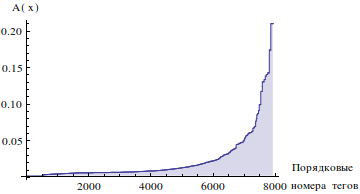
\includegraphics[width=0.5\linewidth]{Dissertation/pics/abstract_words_1}
    \caption{Значения степени абстрактности}
  \end{minipage}
  \label{img:abst_1}
\end{figure}

\begin{figure}[ht]
  \begin{minipage}[ht]{1.0\linewidth}\centering
    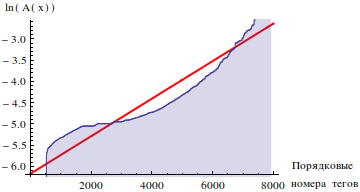
\includegraphics[width=0.5\linewidth]{Dissertation/pics/abstract_words_2}
    \caption{Значения логарифмов степени абстрактности}
  \end{minipage}
  \label{img:abst_2}
\end{figure}


Формулу, определяющую оптимальное значение степени абстрактности p, в окрестность которого попадёт максимальное число искомых тематических тегов, можно представить в следующем виде:

$$p=\exp{M(\{\log{x}|x = \underset{y}\max{(A(y)|y\in p), p \in P})}$$,

где $P$- множество всех наборов ключевых слов, $A(y)$ - абстрактность ключевого слова $y$, $M(x)$ - среднее значение среди $x \in X$

После определения параметра $p$ остается выбрать интервал, содержащий значение $p$.  Например, можно отступить в обе стороны от $p$ на $\epsilon$ и обозначить множество тегов таких, что $A(x) \in [p − \epsilon,p + \epsilon]$, множеством тематических тегов.

\subsubsection{Тестовые испытания модели определения абстрактности и тематических тегов} \label{abstr_test}

В настоящем разделе результаты тестовых испытаний программной реализации алгоритмов определения степени абстрактности ключевого слова, тематических тегов и тематики документа, а также описываются методы предварительной обработки исходных данных и исправления ошибок.  В качестве таких тестовых данных в работе использован корпус ключевых слов научных публикаций. Коллекция представляла собой вручную составленные списки ключевых слов для публикаций технического и гуманитарного профиля, полученные из различных источников, включая сеть Интернет. По этой причине в этих данных присутствовали ошибки и неточности, полученные при их формировании.

По причине того, что данные для тестовых испытаний вводились людьми вручную, было необходимо провести предварительную обработку данных. Предобработка данных - необходимая мера для увеличения точности работы алгоритмов. К мерам, которые применялись для улучшения качества тестовых данных относятся следующие:

\begin{itemize}
    \item все ключевые слова переводились в нижний регистр;
    \item самые популярные из аббревиатур вручную сопоставлялись со своими развёрнутыми формами;
    \item использовалось несколько разделительных символов;
    \item длинные строки без разделителей разделялись по символам пробелов;
    \item в ключевом слове убирался дефис, если уже существует такое же слово без дефиса.
\end{itemize}

При этом замечается, что длинные строки без разделителей в действительности могут представлять собой единственное ключевое слово:

\textbf{[оценка экономического косвенного эффекта от проекта информатизации]}.\

Или же набор ключевых слов, разделенных по пробелу

\textbf{[шахта метан утилизация газогенераторная станция]}.\

По причине того, что длинные ключевые слова встречаются в данных пренебрежимо мало и в соответствующих вершинах построенных графов мало связей, такие длинные одиночные ключевые слова расценивались как множество однословных ключевых слов.

Далее приведен список самых популярных ключевых слов:

\textbf{наночастицы, инновации, метод конечных элементов, механические свойства, динамика, наноструктуры, прочность, научный потенциал, удар, структура, остаточные напряжения, компьютерное моделирование, управление, модель, оптимизация, мониторинг, образование, математическое моделирование, математическая модель, моделирование}

Популярность некоторых из этих слов является следствием высокой степени абстрактности (моделирование), но некоторые из них попали в список, потому что некоторая тема может быть популярной (по крайней мере, в рамках данной коллекции). По этой причине теги, относящиеся к этой тематике, могут часто быть использованы в списке ключевых слов (наноструктуры, метод конечных элементов). Способы отделения друг от друга тегов этих двух видов рассматриваются в следующем разделе. Однако, уже сейчас видно, что наивный алгоритм подсчёта количества вхождений тега в коллекцию не даёт необходимого результата.

Далее на Рис. \ref{img:abstr_hist} показано количество наборов, обладающих соответствующей долей неуникальных тегов (т.е. тех тегов, которые упоминаются хотя бы в двух наборах из коллекции). Другими словами, для каждого набора подсчитан процент неуникальных ключевых слов и по этим данным построена гистограмма. Важно отметить, что именно неуникальные теги дают возможность дальнейшего анализа. Если бы наборы в основном состояли из уникальных тегов, то использование графов и статистического анализа не привело к достижению каких-либо результатов. Самое популярное значение доли неуникальных тегов - 1.0. Этот факт означает, что теги всех наборов этой категории не являются уникальными, несмотря на то, что коллекция состоит по большей части из уникальных тегов. Примером такого набора является:

\textbf{[образование, наука, высшая школа, идеология, математика, филология, история, педагогика, биология]}

\begin{figure}[ht]
  \begin{minipage}[ht]{1.0\linewidth}\centering
    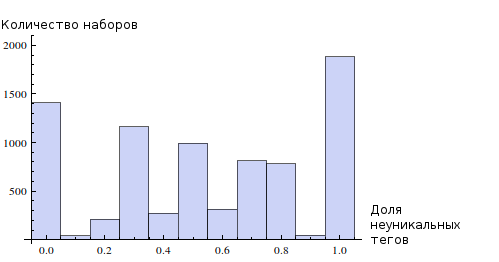
\includegraphics[width=0.5\linewidth]{Dissertation/pics/abstr_hist}
    \caption{Кол-во наборов, с соответсвующей долей неуникальных ключевых слов}
  \end{minipage}
  \label{img:abstr_hist}
\end{figure}

Зачастую теги наборов такого типа являются очень абстрактными понятиями, что в редких случаях позволяет понять тематику документа. Второе по популярности значение - 0.0. Оно показывает, что существует много наборов, целиком состоящих из уникальных тегов. Причины возникновения таких наборов состоят в следующем:

\begin{itemize}
    \item ключевые cлова являются слишком узкоспециализированными, например - \textbf{фемтосекундная спектроскопия, лазерные солитоны, дипирролилметаны, подповерхностный радиолокатор};
    \item ключевые слова представлены на другом языке - \textbf{control, sensitivity, equilibria, chaos}.
\end{itemize}

Следует однако отметить, что основная причина именно в узкой специализации тегов.

Между значениями $0.0$ и $1.0$ находится более половины всех наборов. Средняя доля неуникальных тегов по всей коллекции равна $0.53$, то есть, в среднем половина тегов набора встречается в некотором другом объекте коллекции. Типичный набор состоит из нескольких абстрактных тегов, указывающих на общее направление работы и дисциплины, и нескольких тегов, позволяющих понять, о чем конкретно представленный документ.

Исходя из перечисленных выше факторов, представляется возможным изучать методы автоматического определения тематики документа и особенности алгоритмов ассоциативного поиска. При этом логичным инструментарием для решения поставленных задач являются графы, которые были введены в предыдущем разделе. Такие графы будут иметь достаточную связность для дальнейшего анализа и возможности примения алгоритмов, которые представлены в предыдущих разделах.

Для графа ключевых слов, построенного по данным, были определены компоненты связности и вычислены их размеры. Общее число компонент связности - 1856, что, очевидно, очень много для графа из 17428 вершин. Однако, как показывает график на рис.\ref{img:abstr_hist_2} зависимости номера компоненты и её размера (ось ординат логарифмическая), наибольшая компонента связности содержит более половины всех тегов (11558), а вторая по величине имеет лишь 92 вершины. Начиная с 38 позиции, в компонентах содержится менее 10 вершин.

\begin{figure}[ht]
  \begin{minipage}[ht]{1.0\linewidth}\centering
    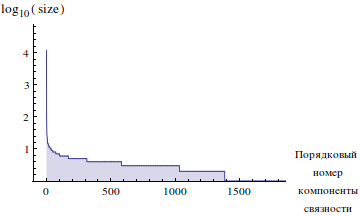
\includegraphics[width=0.5\linewidth]{Dissertation/pics/abstr_hist_2}
    \caption{Распределение размеров компонент связности}
  \end{minipage}
  \label{img:abstr_hist_2}
\end{figure}

\subsubsection{Дополнительный тестовый набор данных}
По причине того, что имеющийся набор данных недостаточно велик, был разработан алгоритм сбора информации о ключевых словах научных статей из сети Интернет. Для этого был использован AP I поисковой системы Яндекс, представляющей функциональные возможности получения поисковой выдачи по запросу. Суть алгоритма в следующем.  

На вход алгоритма подается одно ключевое слово <KEYWORD>. В поисковую систему отправляется запрос вида <<mime:pdf keywords: /5 <KEYWORD> >>. Этот запрос означа- ет, что необходимо найти документы формата pdf, в которых после слова «keywords:» на расстоянии не более 5 слов находится заданное слово <KEYWORD>. Поисковая система возвращает сниппеты релевантных документов. Ожидается, что значительная часть сниппетов будет содержать список ключевых слов некоторых научных статей. Производится парсинг сниппетов, выделяются кортежи ключевых слов. Собранные ключевые слова добавляются в множество ключевых слов. Тег-запрос добавляется в список использованных ключевых слов. Новое ключевое слово <KEYWORD> выбирается из разности множества всех ключевых слов и множества использованных. Действия алгоритма повторяются до тех пор, пока не будет собрана база ключевых слов достаточного размера.

Недостатком программной реализации представленного алгоритма является то обстоятельство, что внешняя поисковая система ограничивает количество запросов в день. По этой причине сбор необходимых данных занимает продолжительное время. Чтобы ускорить процесс, для каждого запроса выкачивается максимально возможное число документов. Как следствие, ключевые слова, по которым строился запрос, встречаются гораздо чаще в собранном множестве ключевых слов. Такой перекос негативно влияет на статистические параметры выборки и ухудшает качество работы реализаций алгоритмов. Другой недостаток состоит в том, что если брать слишком большое число документов, то хвост выдачи становится менее релевантен и в выборку добавляются <<мусорные>> данные.

Тем не менее алгоритм решает важную задачу - восполняет недостаток данных. С помощью программной реализации было собрано более 380000 наборов ключевых слов. Для них были проведены методы предобработки данных, описанные в предыдущем пункте. Дополнительно к этому удалялись наборы без разделителей. Вероятнее всего, такие наборы - это обычные предложения со словом keywords, а также наборы, в которых ключевые слова имеют слишком малую длину (обычно в такие сниппеты попадали инициалы авторов статей). Далее это множество данных обозначается как данные из Веб, а первая коллекция именуется чистыми данными.

\subsubsection{Результаты тестовых испытаний модели определения абстрактности слова}

Самые абстрактные слова, полученные при использования программной реализации описанного выше алгоритма на чистых данных:

\textbf{моделирование, модель, образование, оптимизация, управление, структура, математическая модель, математическое моделирование, мониторинг, прогнозирование, инновации, эффективность, методика, личность, прочность, эксперимент, оценка, история, методы, развитие, анализ, здоровье, инновационная деятельность, культура, качество, свойства, модернизация, синтез, надежность, самоорганизация, адаптация, конкурентоспособность, интеграция, студенты, безопасность, компетенции, взаимодействие, технологии, диагностика, наука, государство, компьютерное моделирование, инновационное развитие, устойчивость, компетентностный подход, динамика, технология, высшая школа, нано-
частицы, метод конечных элементов.}

В целом получены неплохие результаты по экспертной оценке. Из выделенных слов значительную часть можно назвать абстрактными в некотором смысле. Смешивание помогло избавиться от явных выбросов в каждом из алгоритмов и несколько усреднить результат. Тем не менее, добиться заметного повышения качества не удалось, поскольку представленные алгоритмы имеют одну природу и решают схожие задачи. По этой причине они зачастую ошибаются на некоторых данных одновременно, что влечет за собой ошибку в результатах работы общего алгоритма.

Результаты работы программной реализации алгоритма на данных из Веб:

\textbf{development, data mining, environment, evaluation, model, management, machine learning, modelling, growth, reliability, neural networks, design, stability, learning, security, uncertainty, clustering, education, performance, modeling, optimization, simulation}

Для этого набора получены схожие по качеству результату. Однако можно заметить, что некоторые слова продвигаются вверх из-за того, что они были использованы в запросах. Таким словом, например, является термин «machine learning», который не должен был войти в множество абстрактных слов.

\subsubsection{Результаты тестовых испытаний модели определения тематических тегов}
Значение искомого параметра $p$ в описанном ранее алгоритме оказалось равным $0.0122$.  На чистых данных, для удобства тестирования был выбран интервал $[0.012, 0.013]$. Теги, которые имеют такую степень абстрактности, определены как тематические. Таких ключевых слов обнаружено $65$. В приложении \ref{AppendixB} приводится полный список определенных тематических тегов. Таким образом, алгоритм определил $65$ тегов, из которых $19$ при любых обстоятельствах являются тематическими потому, что это название дисциплин и направлений науки. Еще $13$ тегов субъективно можно считать тематическими. Таким образом точность результата составляет $49.2\%$.

\subsection{Определение смысловой близости для решения задачи поиска эксперта} \label{expert_search_wordsim}
Постановка и решение задачи поиска эксперта рассматривается в главе \ref{expert_search}. Для ее решения возникает необходимость вычислять похожесть между наборами ключевых слов, характеризующих потенциальных экспертов, с ключевыми словами запроса. Для этого, в свою очередь, разработана базовая процедура для определения близости пары ключевых слов, использующая методы и идеи, которые описаны в настоящей главе.

Вычисление смысловой близости пары ключевых слов также основывается на построении графа ключевых слов, введенного в (???). Вершины этого графа соответствуют ключевым словам, а взвешенные ребра отражают факт вхождения слов в один набор. Другим важным понятием является уровень абстрактности ключевого слова, который описан в главе (???). Под абстрактностью понимается степень общности значения слова. Алгоритм определения степени абстрактности по ключевому слову описан в (???). Для вычисления смысловой близости пары ключевых слов используются следующие далее соображения.

\begin{itemize}
    \item \textbf{Чем ближе друг к другу находятся теги в графе, тем больше они схожи по смыслу.} Другими словами, значение семантической близости обратно пропорционально кратчайшему расстоянию между вершинами в графе. За вес ребра принято число наборов из корпуса, в которые входят оба тега. Если $w(i, j) = |{p \in W_X | i \in p \wedge j \in W_X}|$ ­ вес ребра ($W_X$ - множество всех наборов ключевых слов информационной системы), то за длину ребра принята величина $l_0(i, j) = \frac{1}{1+\log(w(i,j))}$ , где $i$, $j$ ­ смежные вершины. Для случая $i = j$ положим $l_0(i, i) = 0$. Следует отметить, что от функции $l_0(i, j)$ достаточно потребовать лишь обратной зависимости от функции $w(i, j)$ . Тем не менее, описанная выше формула позволяет получить лучший результат, чем, например, наивная формула $\frac{1}{w(i,j)}$.
    \item \textbf{Необходимо использовать только статистически важные связи в графе.} Набор ключевых слов к научной публикации не обязан состоять из похожих по смыслу слов. Например, в одном наборе (<<космический аппарат>>, <<упругие элементы>>, <<процесс отделения>>). Замечается, что ключевые слова <<космический аппарат>> и <<упругие элементы>> не должны обладать сильной семантической связью. Поэтому вводится условие: если количество совместных появлений пары тегов меньше порогового значения $t$ , то такая связь в графе не учитывается. Исключением являются те ребра, удаление которых приводит к увеличению числа компонент связности в графе ключевых слов.
    \item \textbf{Пара слов с более высокими степенями абстрактностей должна обладать меньшим значением семантической близости, чем пара узкоспециальных слов.} В качестве примера рассмотрим следующую ситуацию: пара абстрактных по значению тегов («динамика», «кинематика») и пара более узкоспециальных тегов («прибыль», «доход») могут располагаться на одном расстоянии друг от друга в графе. Однако видно, что пара («прибыль», «доход») явно должна иметь большее значение смысловой близости, потому что оперирует более узкоспециализированными тегами. Исходя из этих соображений можно предположить, что семантическая близость должна зависеть от уровней абстрактностей сравниваемых ключевых слов.
    \item \textbf{Пути графа, проходящие через слова с более высокой степенью абстрактности, должны учитываться с меньшим весом.} Слова, обладающие более широким значением, имеют больше связей с другими словами графа. Это обстоятельство приводит к тому, что существует множество пар узкоспециальных слов, которые явно не являются похожими семантически, однако располагаются при этом близко друг к другу в графе. Обычно такое происходит, если пара слов имеет общую вершину с высокой степенью абстрактности. Например, пара тегов («ленивые вычисления», «оценка максимального правдоподобия») находятся близко друг к другу из­за их связей с тегом «машинное обучение», который является более общим понятием. Можно при этом заметить, что на самом деле слова этой пары далеки друг от друга семантически. По этой причине возникает необходимость «перевзвесить» ребра графа. Обозначим степень абстрактности ключевого слова $x$ за $A(x)$. Величина $A(x)$, исходя из введенного в главе (???) определения, не превышает  1. Положим теперь длину ребра равной $l(i, j) = \exp(\frac{l_0(i, j)}{\log(A(i))\log(A(j))})$. Таким образом, чем выше степени абстрактности вершин, инцидентных данному ребру, тем больше длина этого ребра. Длина кратчайшего пути между вершинами $v_x, v_y$ принята за $L(v_x,v_y)$ . Экспонента в формуле делает значение $l(i, j)$ не меньшим, чем 1.
    \item \textbf{Чем больше различных связей (путей) между вершинами в графе, тем больше уровень семантической близости.} При этом дополнительную информацию дают веса ребер. Это следует из того, что если два тега связаны тяжелым ребром или путь между ребрами имеет большой вес, то такие теги будут более близки по смыслу, чем аналогичная пара с легкими ребрами. В этой связи возникает необходимость решения задачи определения максимального потока между двумя вершинами графа. В классической постановке требуется для пары вершин, называемых источником и стоком, транспортной сети найти такой поток из источника в сток, что его величина будет максимальна. На граф тегов эта задача переносится очевидным образом, если ребра принять за двунаправленные, а за пропускную способность ребра ­ его вес. При этом пропускная способность считается отдельно для каждого из направлений. Пусть максимальный поток между вершинами $v_x, v_y$ равен $MaxFlow(v_x, v_y)$. Максимальной вместимостью вершины назовем сумму весов ребер, входящих в нее. Обозначим максимальную вместимость вершины $i$ за $C(i)$. Тогда за $F(v_x,v_y)$ примем величину, равную $\frac{MaxFlow(v_x,v_y)}{min(C(v_x), C(v_y))}$. В этом случае $F(v_x,v_y)$ показывает, насколько использована пропускная способность канала между вершинами. Максимум, равный единице, достигается, если пропускная способность использована полностью. В частности, $F(vx,vx) = 1$.
\end{itemize}

Учитывая перечисленные выше cоображения, формула близости между парой ключевых слов $x$ и $y$ вводится следующим образом:

$$ WordSim_{expert}(x, y) = \frac{F(v_x, v_y)}{L(v_x, v_y)}, $$

где $v_x$ и $v_y$ - пара вершин в графе ключевых слов, соответствующая ключевым словам $x$ и $y$.


\subsection{Тестовые испытания} \label{test_sect}
В настоящем разделе описаны результаты тестовых испытаний программных реализаций описанных ранее алгоритмов. В качестве тестовых данных были использованы корпусы ключевых слов для научных публикаций, собранных из сети Интернет. Использовалась также информация из социальной сети Вконтакте, а именно - были выкачаны посты (публичные сообщения из групп и страниц пользователей), часть из которых помечены хэштегами. В процессе сбора данных проводился парсинг текстовых данных на предмет наличия в них наборов ключевых слов. Точное решение этой задачи не является предметом исследования данной работы (???), поэтому для парсинга данных были использованы наивные подходы, которые, тем не менее, позволяют собрать корпус достаточного размера и качества  для проведения дальнейшего анализа.
В конечном итоге собрано два объемных набора данных:
\begin{itemize}
    \item 329.000 наборов для русского языка;
    \item 3.069.000 наборов хэштегов из сети Вконтакте.
\end{itemize}
Далее приведены примеры наборов ключевых слов из обоих источников. Наборы ключевых слов научных публикаций:

    \textbf{[топонимический концепт, языковое сознание, когнитивная база, прецедентность, апеллятивация]}\

    \textbf{[вариабельность сердечного ритма, гребля на каноэ, вегетативный тонус]}\
    
    \textbf{[архитектуры, деформации, геологическая среда, сфера взаимодействия]}

Наборы хэштегов из социальной сети:

    \textbf{[electro\_pop, dance, fresh, music, new\_zealand]}\

    \textbf{[vitaminhealth, oxygenwater, waterhealth]}\

    \textbf{[bodyfan, питание, bodyfanпитание, bodyfanmotivation, motivation, bodybuilding, фитнес, gym, спорт, мотивация, зож]}

\subsubsection{Определение семантической близости с использованием графов ключевых слов}
Программные реализации описанных в предыдущих главах алгоритмов были применены к собранным данным. Далее на рисунке \ref{img:sim_1} представлены ближайшие соседи для слов <<федерация>> и <<регионы>> в графе ключевых слов.

\begin{figure}[ht]
  \begin{minipage}[ht]{0.49\linewidth}\centering
    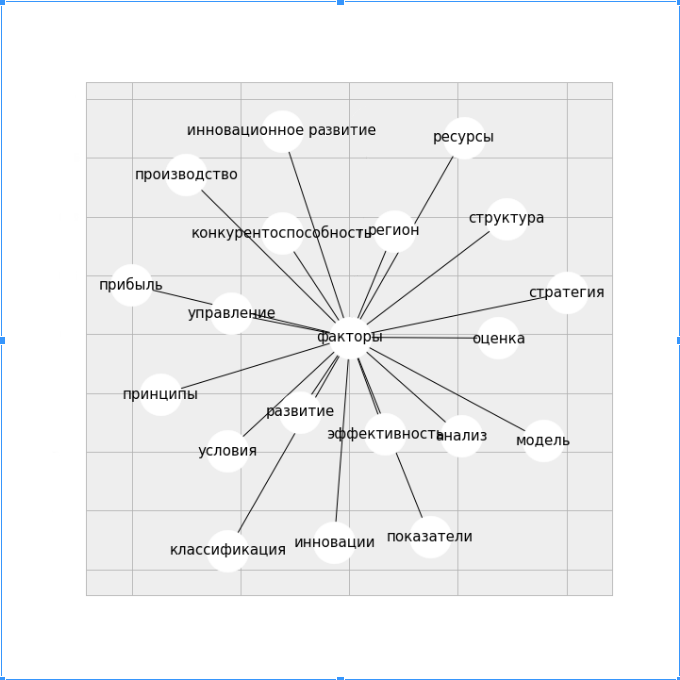
\includegraphics[width=1.0\linewidth]{Dissertation/pics/factory_sim} \\ а)
    \caption{Соседи вершины <<факторы>> в графе ключевых слов}
  \end{minipage}
  \hfill
  \begin{minipage}[ht]{0.49\linewidth}\centering
    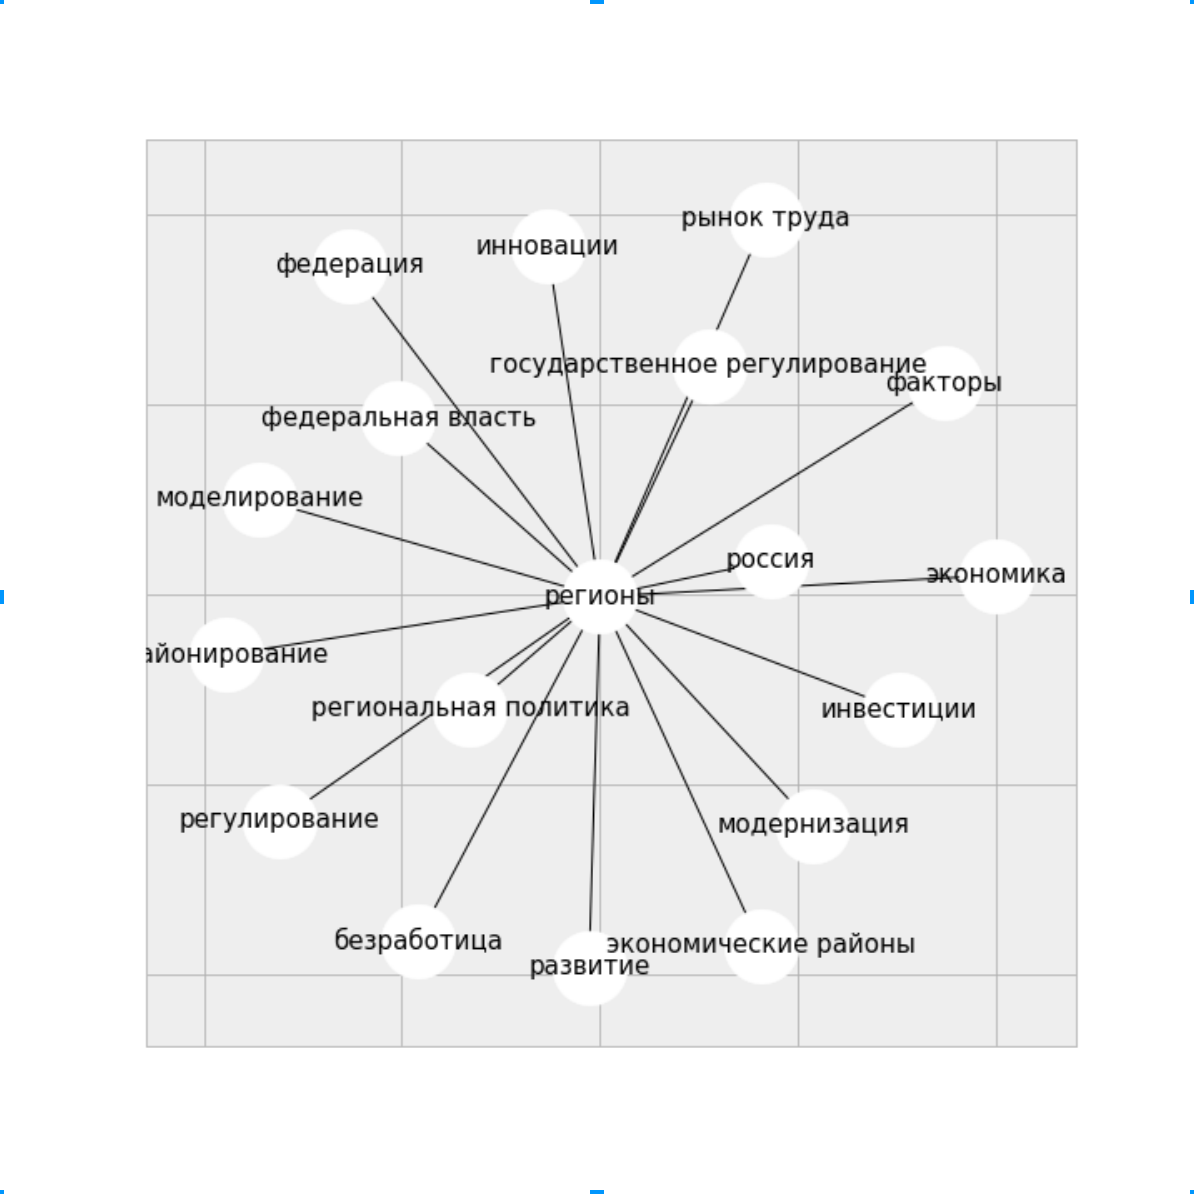
\includegraphics[width=1.0\linewidth]{Dissertation/pics/regiony_sim} \\ б)
    \caption{Соседи вершины <<регионы>> в графе ключевых слов}
  \end{minipage}
  \label{img:sim_1}
\end{figure}

На рисунках выше видно, что графа ключевых слов не хватает для определения семантической близости пары слов: видно, что существуют связи такие, как <<факторы-модель>>, <<регионы-экономика>>, которые не обладают явной смысловой связью. Применение методов построения усеченного контекстного графа дает значительное улучшение качества классификации пар ключевых слов на семантически близкие и далекие. Далее указаны примеры найденных пар ключевых слов, близких по смыслу:

\textbf{β-адреноблокаторы   -   бета-адреноблокаторы}

\textbf{новые виды   -   новый вид}

\textbf{орви   -   острые респираторные вирусные инфекции}

\textbf{текущий уровень информационной безопасности   - политика информационной безопасности}

\textbf{умения   -   навыки}

\textbf{образное мышление   -   художественный вкус}

\textbf{хехцир   -   khekhtsyr}

\textbf{рынок банковских услуг   -   банковский рынок}

\textbf{тромболизис   -   тромболитическая терапия}

\textbf{параллельные алгоритмы   -   параллельное программирование}

\textbf{феминность   -   фемининность}

\textbf{полином  -  многочлен}

\textbf{корень  -   корни}

\textbf{primerun  -  примерун}

\textbf{fvk  -  fotovideoclub}

\textbf{еврореволюция  -   єврореволюція}

\textbf{silk\_plaster    -  шелковая\_штукатурка}

Интересным фактом является определение похожих слов для заданного многозначного слова. В то время как граф в графе ключевых слов соседями для слова <<орган>> являются слова <<государство>>, <<сибирь>>, <<контроль>>, <<циркуляция>>, <<управление>>, в контекстном графе ближайшими являются слова <<музыковедение>>, <<организм>>, <<отклонение>>, <<делегирование полномочий>>, <<объект контроля>>. Таким образом восстанавливается не только значение слова, связанное с юриспруденцией, но и близкие слова для значения из области музыки (<<музыковедение>>) и биологии (<<организм>>).

На рисунке \ref{img:sim_2} изображены несколько ближайших контекстно близких слов для слова <<студенты>> (отмечается, что полное множество соседей вершины слишком велико, чтобы его изобразить):

\begin{figure}[ht]
  \begin{minipage}[ht]{1.0\linewidth}\centering
    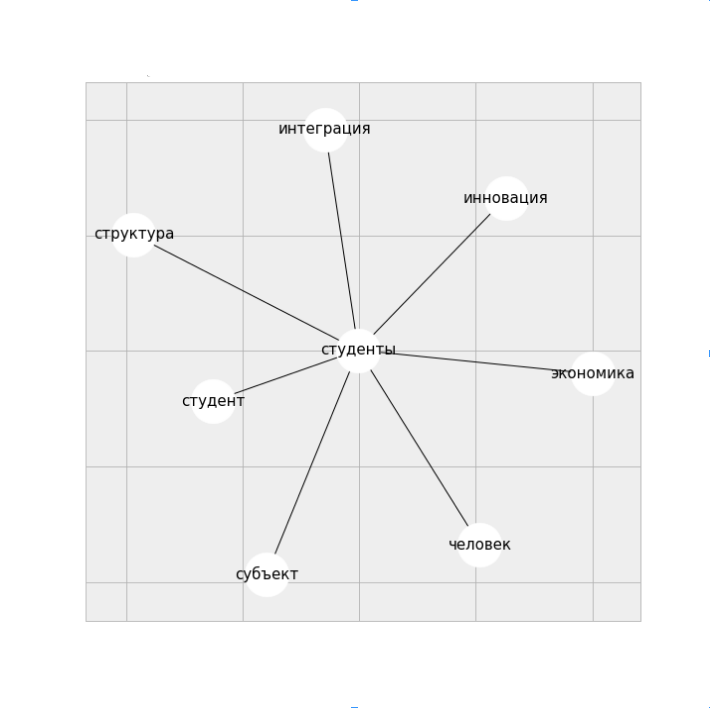
\includegraphics[width=1.0\linewidth]{Dissertation/pics/students_sim}
    \caption{наиболее близкие слова для слова <<студенты>> в контекстном графе}
  \end{minipage}
  \label{img:sim_2}
\end{figure}


\subsubsection{Построение кластеров семантически похожих ключевых слов} \label{clustering_section}

Описанный ранее алгоритм кластеризации контекстного графа позволяет удалять недостаточно надежные связи между словами, полученные с помощью алгоритма определения близости по контекстному графу, и, наоборот, добавлять новые ребра между семантически похожими парами слов. 

Кластер для слова <<студенты>> изображен на рисунке \ref{img:clust_1}

\begin{figure}[ht]
  \begin{minipage}[ht]{1.0\linewidth}\centering
    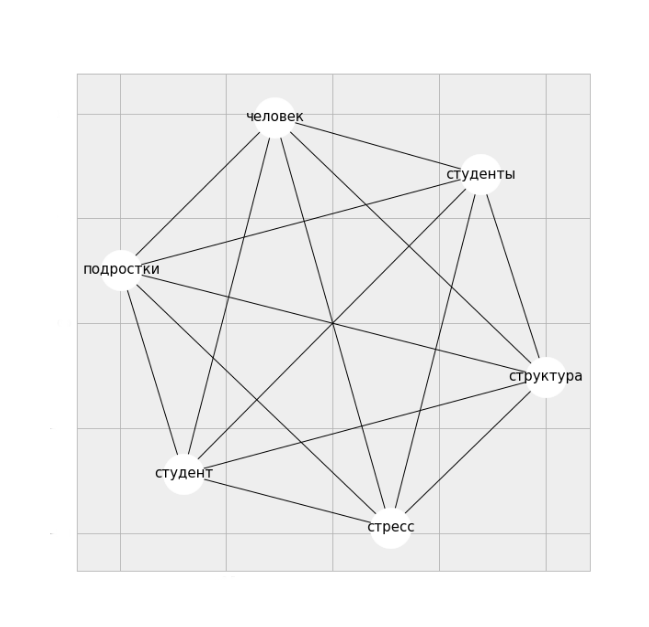
\includegraphics[width=1.0\linewidth]{Dissertation/pics/students_cluster}
    \caption{кластер, содержащий слово <<студенты>>}
  \end{minipage}
  \label{img:clust_1}
\end{figure}

Можно заметить, как в результате кластеризации были разорваны связи <<студенты-экономика>>,  <<студенты-инновации>>, вместо которых на первый план вышли связи <<студенты-подростки>>. Отмечается также, что выбранный метод кластеризации графа может допускать ошибки. Например, в случае с парой <<студенты-структура>>, которая была как в усеченном контекстном графе, так и в кластере слова студент.

Для интегральной проверки качества была выбрана следующая методика.

\begin{enumerate}
    \item Набирается набор пар ключевых слов, для которых можно  определить их высокий уровень семантической близости посредством детерминированного алгоритма (положительные примеры). Пара слов определяется близкой по смыслу, если выполняется хотя бы одно из условий:
    \begin{enumerate} 
        \item одно ключевое слово является аббревиатурой для другого;
        \item расстояния Левенштейна между парой невелико.
    \end{enumerate}
    \item К зафиксированным семантически похожим парам слов добавляются отрицательные примеры, т.е. пары слов, которые не являются близкими по смыслу. Для этого проводятся следующие шаги:
        \begin{enumerate}
            \item если пара слов $(a,b)$ определена на первом шаге как пара похожих слов, то для слова aберется $k$ случайных соседей $c_1, c_2, \dots,c_k$ из графа ключевых слов на расстоянии, не превышающем 2; 
            \item все пары $(a,c_i)$ определяются как отрицательные примеры.
        \end{enumerate}
    \item Положительные и отрицательные примеры составляют тестовую выборку. После чего для всех пар тестовой выборки вычисляется близость, по формулам описанным выше, а также подбирается порог, по которому в зависимости от вычисленного значения близости пара относится либо к классу семантически близких пар, либо к классу семантически далеких.
    \item По оценкам классификатора и тестовой выборке считается F-мера, которая и является показателем качества алгоритма.
\end{enumerate}

В результате тестирования программной реализации алгоритма получено высокое  по отношению к реализованным в [???] алгоритмам значение F-меры - 0.82. Проведение аналогичного теста для алгоритма определения близости лишь с помощью анализа частотности встречаемости пары слов дает результат 0.67, таким образом, методы, описанные в данной работе существенно улучшают качество определения семантической похожести. Отмечается, что выбранный способ тестирования имеет очевидный недостаток: среди положительных примеров очень редко встречаются пары смысловых синонимов, напротив, они могут попадать в пары отрицательных примеров. Тем не менее, по экспертной оценке увеличение качества на описанной ранее тестовой выборке влечет улучшение качества классификации и более сложных пар ключевых слов, таких как  пар <<синоним>>-<<синоним>> или <<слово>>-<<перевод слова на другой язык>>.

\subsubsection{Тестирования алгоритмов определения абстрактности слова}
Самые абстрактные слова, полученные при использования программной реализации
описанного выше алгоритма на чистых данных:

моделирование, модель, образование, оптимизация, управление, структура, математическая модель, математическое моделирование, мониторинг, прогнозирование, инновации, эффективность, методика, личность, прочность, эксперимент, оценка, история, методы, развитие, анализ, здоровье, инновационная деятельность, культура, качество, свойства, модернизация, синтез, надежность, самоорганизация, адаптация, конкурентоспособность, интеграция, студенты, безопасность, компетенции, взаимодействие, технологии, диагностика, наука, государство, компьютерное моделирование, инновационное развитие, устойчивость, компетентностный подход, динамика, технология, высшая школа, наночастицы, метод конечных элементов.

В целом получены неплохие результаты по экспертной оценке. Из выделенных слов значительную часть можно назвать абстрактными в некотором смысле. Смешивание помогло избавиться от явных выбросов в каждом из алгоритмов и несколько усреднить результат. Тем не менее, добиться заметного повышения качества засчет этого не удалось, поскольку представленные алгоритмы имеют одну природу и решают схожие задачи. По этой причине они зачастую ошибаются на некоторых данных одновременно, что влечёт за собой ошибку в результатах работы общего алгоритма.

Результаты работы программной реализации алгоритма на данных из Веб:

development, data mining, environment, evaluation, model, management, machine learning, modelling, growth, reliability, neural networks, design, stability, learning, security, uncertainty, clustering, education, performance, modeling, optimization, simulation

Для этого набора получены схожие по качеству результату. Однако можно заметить, что некоторые слова продвигаются вверх из-за того, что они были использованы в запросах. Таким словом, например, является термин «machine learning» , который не должен был войти в множество абстрактных слов.

\subsubsection{Апробация автоматического тематического классификатора}
...
\subsection{Выводы}
По результатам исследований, результаты которых представлены в разделе \ref{test_sect}, построены модели определения близости по корпусу наборов ключевых слов, опирающиеся на методы из теории графов. Для данных моделей представлены алгоритмы и созданы программные реализации этих алгоритмов. Реализации были протестированы на двух коллекциях наборов ключевых слов и был получен относительно высокий уровень качества результатов. Кроме того, была разработана модель кластеризации ключевых слов, опирающаяся на введенные графовые модели представления коллекций ключевых слов и на построенную по этим графам меру схожести для пары слов. Программная реализация процедуры кластеризации также протестирована, для нее был получен высокий уровень качества определения кластеров схожих ключевых слов.
%\textbf{??? добавить текст про тематический классификатор}
Недостатком работы может являться большое число параметров, которое необходимо настроить. В качестве дальнейшего направления в изучении данной области автор настоящей дисертации считает целесообразным применения методов машинного обучения для построения меры близости между ключевыми словами. Такой шаг поможет избавиться от значительной части параметров описанных в предыдущих главах моделей, предоставив возможность настройки этих параметров в автоматическом режиме.

\section{Использование методов машинного обучения для улучшения модели близости слов} \label{ml_sim}
В настоящей главе рассматриваются методы улучшения качества определения семантической близости для пары ключевых слов с помощью методов машинного обучения с учителем. Далее в тексте подробно описывается сведение рассматриваемой задачи к задаче классификации, то есть к задаче определения целевой метки заданного объекта из заранее сформированного множества меток. Обучение с учителем подразумевают использование обучающей выборки - множества объектов, для которой известны истинные целевые метки. Эта выборка необходима для тренировки модели машинного обучения. Обученная модель машинного обучения применяется к произвольному объекту системы и выдает предсказанную целевую метку.

Сбор обучающего набора данных является обычно трудоемкой и дорогой работой: как правило для процесса требуется как минимум несколько экспертов в направлении, для которого собираются тренировочное множество. Более того, для некоторых задач, в число которых входит и задача определения семантической близости пар ключевых слов, является сложным даже правильно составить инструкцию для экспертов для правильной оценки примеров. Это происходит по причине того, что семантическая близость - субъективная величина и сильно зависит от области применения, контекста, человека и задачи. Например, слово <<стол>> может быть близким по смыслу для слова <<стул>> из бытовых соображений. В то же время если бы эти два слова были синонимами (а следовательно взаимозаменяемыми) в информационной системе, представляющей интернет-магазин, продающий мебель, то имела бы место ситуация, когда пользователь ищет один из этих предметов, а в поисковой выдаче получает другой, что является недопустимым. Рассмотренные в следующих далее разделах алгоритмы сбора обучающего множества призваны разрешить обозначенные проблемы.

Автором настоящей диссертации были разработаны два метода получения обучающих примеров без задействия в процесс экспертов. Первый из них включает в себя набор эвристических алгоритмов создания обучающей выборки. Второй является полностью автоматическим методом и строится исключительно при помощи описанных в предыдущих главах графовых моделей представления данных. Важнейшим преимуществом этого метода является его универсальность и применимость не только к задачам определения семантической близости, но и к любым другим задачам, в которых объекты системы представляются в виде некоторого графа и имеется необходимость в классификации отношений между парой объектов. Также универсальность проявляется в том, что выборка строится непосредственно по данным и не использует никакие внешние источники. Это позволяет определить отношение близости специфичные для конкретной системы. Другое преимущество метода в возможности использовать эффективные модели машинного обучения с учителем, вместо более слабых моделей без учителя, которые, к тому же представляется сложным валидировать без обучающих примеров.

Задача классификации для определения семантической близости пары ключевых слов формулируется следующим образом. Пусть $X=\{x_i\}_{i=1}^N$ - множество пар ключевых слов. $x_i=(x_l,x_r)_i$ - пара ключевых слов, где $x_l,x_r$ - левое и правое слова из пары. $Y={0,1}$ - множество меток. Нулевое значение соответствует отсутствию семантической близости для пары ключевых слов, а единичное, напротив, сильной смысловой связи. Поскольку $Y$ состоит только из двух элементов, то такая задача называется задачей бинарной классификации. $X^l=(x_i,y_i)_{i=1}^l$, где $x_i \in X, y_i \in Y$ - обучающающая выборка. Далее по обучающей выборке строится классификатор $a: X\rightarrow Y$

Процесс сбора обучающей информации является одним из важнейших этапов обучения эффективной модели определения семантической близости. Сложность этого процесса заключается в невозможности точно формализовать для пары ключевых слов отношения <<являются семантически близкими>> и <<не являются семантически близкими>>. Во многих случаях определение смысловой близости зависит от решаемой задачи, поэтому обучающие выборки для одной задачи могут не подходить для обучения моделей из другой. Например, пары ключевых слов <<математика>> и <<математическая статистика>> (связаны отношением гиперонимии (<<математическая статистика>> является разделом <<математики>>), что влечет некоторую смысловую близость между понятиями. C другой стороны, если рассматривать задачу поиска документов системы по ключевым словам, то при заданном пользователем запросе <<информатизация,математика,вектор информатизации,информационные технологии,mathematica>>.  Для данного запроса ключевое слово <<математическая статистика>> не подходит по контексту данного запроса, кроме того, это ключевое слово является более узким по смыслу, чем <<математика>> и поэтому шансы пользователя получить релевантные запросу документы минимальны: если даже пользователь предполагал какую-то более узкую область, нет никаких оснований полагать, что это именно <<математическая статистика>>, а не, например, <<вычислительная математика>>. Обратная ситуация, когда пользватель ввел запрос <<математическая статистика, статистические тесты>>, то поиск в документах предположительно синонимичного слова <<математика>> также может привести к ухудшению выдачи: в результате этого действия, в выдачу вероятно попадут документы слишком общего смысла, такие как статьи про математику как науку.

Другим примером неоднозначности в определении семантической близости может служить различия в тематической направленности систем, в которых используются модели определения смысловой близости. Для наукометрических систем пара ключевых слов <<математическая статистика>> и <<вычислительная математика>> вряд ли должны иметь большое значение метрики смысловой близости, потому что в рамках такой системы эти два понятия представляют два совершенно различных направления математики. В то же время в системах более общей направленности, где могут присутствовать документы любого рода (а не только научные публикации), данная пара ключевых слов должна иметь более высокий уровень семантической похожести, поскольку для такой системы все термины относительно небольшого раздела <<математика>> могут считаться близкими по смыслу.

Качество модели определения семантической близости в данном случае целиком определяется двумя составляющими: параметрами обучающей выборки (качеством, разнообразием и количеством обучающих примеров) и эффективностью выбранного алгоритма машинного обучения. 

Лучшим алгоритмом для решения поставленной задачи бинарной классификации является модель градиентного бустинга на решающих деревьях XGBoost \cite{xgboost}. В ходе обучения происходит последовательное построение композиции решающих деревьев, каждое следующее дерево при этом стремится максимально уменьшить ошибку уже построенной части ансамбля. Анализ эффективности выбранной модели, сравнения модели XGBoost с другими существующими моделями и тестовых испытания представлены в следующих далее разделах. 

\subsection{Методы формирования обучающей выборки}
В данном разделе описывается два разработанных способа получения обучающего набора данных. Первый из них использует различные эвристические идеи о том, как с помощью простых детерминированных процедур и, в некоторых случаях, внешних открытых наборов данных получать примеры близких по смыслу пар ключевых. Такие методы имеют высокий уровень точности, но слабое покрытие пространства пар ключевых слов системы. Второй способ заключается в использовании теоретико-графовых алгоритмов для, способных выдавать примеры семантически близких и далеких пар объектов, основываясь на графовой структуре представления данных.

\subsubsection{Эвристические методы}
Идейно различаются два типа алгоритмов сбора обучающей выборки. Первый из них заключается в использовании некоторых внешних словарей и дальнейшая фильтрация этих словарей по тем словам, которые присутствуют в информационной системе. Второй способ сначала использует некоторый генеративный алгоритм (например, составляется большое множество пар ключевых слов, которые встретились внутри одного набора). Далее это множество фильтруется с помощью некоторого алгоритма и те пары, которые прошли фильтрацию, объявляются близкими по смыслу. Примером такого алгоритма может быть алгоритм, считающий расстояние Левенштейна. Если редакторское расстояние не превосходит 1, то слова имеют очень схожее написание и  весьма вероятно, что они близки по смыслу. Такая процедура фильтрует значительную часть пар, но те пары, которые прошли фильтрацию, почти всегда  имеют высокую степень смысловой близости. Таким образом каждый такой фильтр получает примеры близких по смыслу пар слов с высокой точностью, но низкой полнотой. 

Были разработаны следующие эвристические методы сбора обучающей выборки
\begin{itemize}
    \item Поиск простых аббревиатур. Ключевые слова системы разделяется на понятия, содержащие ровно одно слово - аббревиатуры, и понятия, содержащие более одного слова- расшифровки аббревиатур. Далее для каждого слова из множества аббревиатур и каждого словаиз множества расшифровок проверяется, действительно ли данная расшифровка является расшифровкой для данной аббревиатуры. Другими словами проверяется, что существуют такие префиксы слов расшифровки, которые могут полностью покрыть аббревиатуру. Если соответствие установлено, то пара аббревиатура-расшифровка добавляется в список пар-кандидатов. Далее к парам-кандидатам приписываются частоты входящих в них ключевых слов. Для каждой аббревиатуры берется не более 5 наиболее частотных вариантов расшифровок. Пары, прошедшие данную фильтрацию, формируют окончательное обучающее множество аббревиатур;
    \item поиск скобочных аббревиатур. Иногда при написании ключевых слов-аббревиатур в скобках указывается правильная расшифровка для данной аббревиатуры. Это позволяет собрать дополнительные пары аббревиатура-расшифровка для обогащения множества обучающих примеров;
    \item поиск разных форм одного слова. С помощью пакета обработки естественного языка NLTK для каждого слова в системе рассматриваются различные его формы. Если одна из форм также присутствует в множестве всех ключевых слов, то пара слово-форма добавляется в обучающее множество;
    \item поиск похожих по написанию слов. Рассматриваются все пары слов, расстояние левенштейна между которыми равно 1. Эти пары добавляются в обучающее множество;
    \item поиск переводов с одного языка на другой. Данный метод использует API сервиса Яндекс.Переводчик и собирает варианты переводов ключевых слов с русского языка на английский;
    \item поиск синонимов в тезаурусе WordNet. Были использованы пары синонимов и пары гипоним-гипероним. Кроме поиска по англоязычным синсетам был использован двухступенчатый подход определения синонимов: русскип слова переводились средствами сервиса Яндекс.Переводчик на английский язык, а затем поиск проводился уже по английским версиям слов;
    \item использование открытых источников синонимов. Из словарей синонимов, доступных в сети Интернет, выделяются те пары, слова которых присутствуют в множестве ключевых слов.
\end{itemize}

Данные методы сбора данных позволяют собрать положительные примеры для обучения, то есть примеры пар ключевых слов, являющиеся семантически похожими. Однако, для правильного обучения модели необходимы также и отрицательные примеры. С помощью небольших модификаций эвристических алгоритмов сбора положительных примеров можно получить алгоритмы для сбора отрицательных примеров. Были использованы следующие идеи:
\begin{itemize}
    \item поиск антонимов в тезаурусе WordNet. Аналогично поиску синонимов был проведен поиск антонимов в базе WordNet. Также были использованы пары слов, расстояние в дереве WordNet между которыми превышает 2;
    \item неправильные расшифровки для аббревиатур. Рассматриваются те аббревиатуры, для которых были найдены правильные расшифровки. Этим аббревиатурам ставятся в пару случайные многословные ключевые слова, которые точно не являются правильными расшифровками;
    \item использование открытых источников антонимов;
    \item случайные пары ключевых слов. Для каждого ключевого слова, для которого в выборке присутствуют положительные примеры, были взяты случайные ключевые слова в пару. На одно слово было сгенерировано не более, чем 10 пар. Данный метод был использован по следующим соображениям. Предполагается, что для каждого ключевого слова существует константное число близких по смыслу ключевых слов. То есть если в достаточно большой информационной системе начинает расти количество ключевых слов, то кол-во слов, похожих на данное слово, не будет расти линейно по числу уникальных слов системы. В то же время количество пар растет квадратично, а количество пар для заданного слова - линейно, а это означает, что если взять для заданного слова в пару случайное слово, то эта пара не будет связана семантически. При этом важным является подбор доли случайных пар. Если эта доля мала, то в выборке не будет достаточного разнообразия отрицательных примеров. Если же доля слишком велика, то случайные пары будут вносить слишком большой вклад в обучение модели, что не является правильным вариантом, потому что в случайные отрицательные пары не настолько качественны, как, например, антонимы из словаря. Оба этих случая приводят к ухудшению качества модели определения семантической близости.
\end{itemize}

В результате работы программных реализаций алгоритмов было собрано 234974 положительных и 1175610 отрицательных примеров.

Обучение моделей на эвристически подобранных выборках имеет заметные недостатки:

\begin{itemize}
    \item Смещение в данных. Для наилучшего обучения классификаторы необходимо, чтобы объекты обучающей выборки выбирались из распределения тех объектов, на которых классификатор будет работать в реальной системе. Рассмотрим данную особенность на следующем тривиальном примере. Допустим, что все пары ключевых слов системы делятся на Аббревиатуры (то есть пара аббревиатура - расшифровка аббревиатуры) и Переводы (слово на русском языке - его перевод на английский). Если Аббревиатур в системе 10\%, то и в обучающем подмножестве должно Аббревиатур должно быть 10\%. Если же аббревиатур при обучении будет значительно больше (например, 70\%), то модель начнет усиленно использовать те факторы, которые повышают ее качество на аббревиатурной части выборки, потому что это лучшим образом оптимизирует функцию потерь. Однако, в момент применения модели, к ней на вход будет поступать только 10\% аббревиатур и 90\% переводов и очень вероятно, что факторы, используемые моделью не будут оптимальны для классификации переводов и тем самым это улучшит качество реальных решаемых задач данным классификатором.  

Другой недостаток смещения заключается в том, что если перегрузить обучающую выборку примерами неправильных переводов, то это негативно отражается на предсказанных уровнях близости во время этапа применения модели. То есть это понизит средний уровень близости между переводами в системе. Это понижение приведет к тому, что если для данного ключевого слова (<<MSU>>) есть и правильная аббревиатура (<<Moscow State University>>), и правильный перевод (<<МГУ>>), то из-за рассмотренной манипуляции с обучающей выборкой, значимость перевода будет понижена. В конечном счете может оказаться, что согласно модели, все аббревиатуры лучше всех переводов. Такое поведение не очевидно и не основывается на реальной работе информационной системы. Такой сценарий возможен, поскольку положительные и отрицательные примеры берутся из разных источников, поэтому степень покрытия ими всего разнообразия пар ключевых слов, а также возможность контролировать нужную долю положительных примеров остается под вопросом;
    \item модель настраивается не под конкретную задачу и не под конкретные данные системы. Если, например, слова <<объединять>> и <<интегрировать>> попали в один внешний словарь синонимов общего назначения, то внутри информационной системы, направленной на изучение технических наук, эти слова определяют две различные математические операции. Также может случиться, что в узкоспециальных областях эти могут являться слишком общими по смыслу, чтобы быть похожими. Примером такой пары может быть <<ураган>> и <<тайфун>>. Для пользователя, например, социальной сети эти слова действительно похожи. Однако, в рамках системы, изучающей различные природные явления, слова имеют важные смысловые отличия. И чем специфичнее тематика системы, чем четче прослеживается различия между словами, который с точки зрения словарей общей направленности, очень похожи;
    \item сложность процесса сбора обучающей выборки. Для каждой системы нужны свои наборы эвристик, что затрудняет внедрение таких классификаторов повсеместно.
    \item ошибки в выборке. По причине того, что частично выборка состоит из случайных примеров, вероятно, что существует небольшое число пар, которые ошибочно промаркированы отрицательными. Это может понизить качество обученной модели. Помимо этого могут возникать ошибки второго рода. Например, если внешний сервис, предоставляющий переводы для слов и фраз допустил ошибку, то в множество положительных примеров попадет неправильный перевод для слова.
\end{itemize}

\subsubsection{Автоматические методы}
Для устранения недостатков, описанных в предыдущей главе, был разработан метод автоматической генерации обучающей выборки. Суть данного метода заключается в использовании графовой структуры данных для получения обучающих примеров.

Первым шагом метода является искусственная модификация текстовых данных. Для этого вводится специальный символ @, который не используется в написании ключевых слов. Далее фиксируется некоторое дискретное распределение. В первой версии программной реализации данного алгоритма было использовано дискретное равномерное распределение из двух значение и далее для простоты основная суть и мотивация алгоритма будут изложены именно для этого распределения.

Рассматриваются ключевые слова, встретившиеся хотя бы $N$ раз в системе. $N$ выбирается таким образом, чтобы отсеять те слова, для которых в системе недостаточно информации, но при этом множество множество  ключевых слов прошедших фильтрацию оставалось достаточным (десятки тысяч слов) для дальнейшего обучения: в сгенерированную выборку попадут только эти слова. В программной реализации параметр $N$ был принят равным $10$. 

Пусть $w_i^k$ обозначает вхождение $i$-го ключевого слова системы в $k$-ый набор ключевых слов. Для каждого вхождения слова $w_i^k$, прошедшего фильтрацию, в наборы ключевых слов, берется число $d$ из выбранного распределения. После этого к вхождению слова $w_i^k$ приписывается суффикс $@d$, то есть добавляется специальный символ @ и ставится число $d$ из распределения. Таким образом, данная операция производит новое ключевое слово. Рассмотрим, например, следующие наборы ключевых слов:

\textbf{[резание металлов, высокоскоростное фрезерование]}\

\textbf{[резание металлов, аморфизация, адгезия, наростообразование]}\

\textbf{[резание металлов, адгезия, высокосоростное фрезерование]}\

После описанной выше процедуры эти наборы ключевых слов могли перейти в:

\textbf{[резание металлов@0, высокоскоростное фрезерование@1]}\

\textbf{[резание металлов@1, аморфизация@1, адгезия@0, наростообразование@1]}\

\textbf{[резание металлов@1, адгезия@0, высокосоростное фрезерование@1]}\

Таким образом, каждое слово $w$, прошедшее первичную фильтрацию по частоте встречаемости, переходит в два новых слова $w@0$ и $w@1$. И во всей коллекции наборов ключевых слов теперь используются модифицированные версии $w@0$ и $w@1$. Это пара слов $w@0$ и $w@1$ является, по сути, одним и тем же словом, и, следовательно, может быть положительным обучающим примеров для выборки. Поскольку слово $w$ в исходных данных встречалось достаточное количество раз. После того, как модифицирован весь объем предоставленных данных, происходит построение описанных в предыдущих главах графов, выполняются процедуры подсчета факторов. Задачей модели машинного обучения в этом случае будет восстановить по графовым связям факт идентичности разных версий одного слова. Если модель успешно обучена искать различные версии одного и того же слова, то при применении модели на реальных данных, появляется возможность классифицировать пары синонимов и, более общо, определять семантическую связь между ключевыми словами.  Это происходит по той причине, что синонимичная пара на самом деле обладает тем же свойством, каким обладает искусственно полученные положительные примеры выборки: при замене одного слова на другое не меняется смысл всего набора. А значит стоит ожидать, что статистические и графовые связи между искусственной парой слов и синонимичной парой во многом похожи.

Но в рамках описанной модели генерации обучающих примеров возникает эффект, из-за которого появляются статистические различия между созданными искуственными парами и настоящими синонимичными словами. Дело в том, что при наивном выборе в равномерного дискретного распределения из двух элементов в качестве генерирующего распределения, зачастую слова $w@0$ и $w@1$ встречаются приблизительно равное число раз. При этом настоящие синонимичные пары таким свойством обладать не обязаны. Например, ясно, что слово "зарплата" будет употребляться гораздо чаще, чем устаревший синоним "жалованье". Поэтому для моделирования искусственной обучающей выборке необходимо взять более сложное распределение. В качестве такового было выбрано геометрическое распределение, поскольку оно позволяет создавать для одного слова несколько различных версий (теоретически ограниченное лишь количеством упоминаний исходного слова в системе), но при этом слова с меньшими значениями индексов будут встречаться чаще из-за природы распределения. То, насколько <<пологой>> получается функция распределения, контролируется параметром $p$ (рис.\ref{img:geom_distr}). Отмечается при этом, что обычно качество собранных данных выше, если значение $p$ достаточно высоко (в интервале $(0.5, 0.9)$). На рис. \ref{img:geom_distr_2} показана гистограмма индексов при генерации модифицированных версий некоторого ключевого слова.

Поскольку теперь каждое исходное слово $w$ может иметь несколько различных модифицированных вариантов $w@0, w@1, ..., w@n, ...$, то это позволяет расширить обучающее множество данных всеми возможными парами из модифицированных вариаций слов: $(w@0, w@1), (w@0, w@2), ... (w@n, w@n+1), ...$. Это позволяет значительно расширить объем обучающей выборки, что приводит к более качественному обучению модели.


\begin{figure}[ht]
  \begin{minipage}[ht]{1.0\linewidth}\centering
    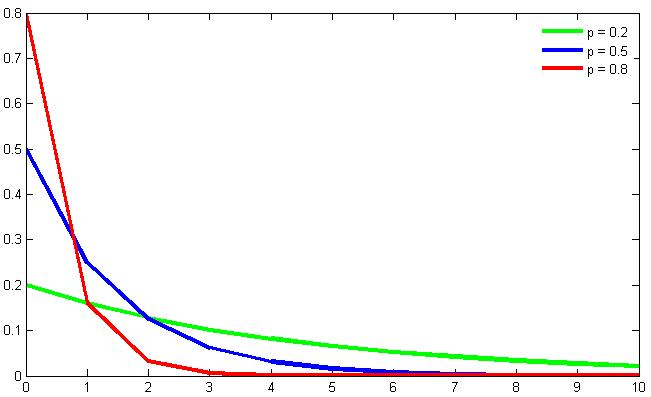
\includegraphics[width=0.7\linewidth]{Dissertation/pics/geom_distr}
    \caption{Плотность геометрического распределения при разных значениях}
  \end{minipage}
  \label{img:geom_distr}
\end{figure}

\begin{figure}[ht]
  \begin{minipage}[ht]{1.0\linewidth}\centering
    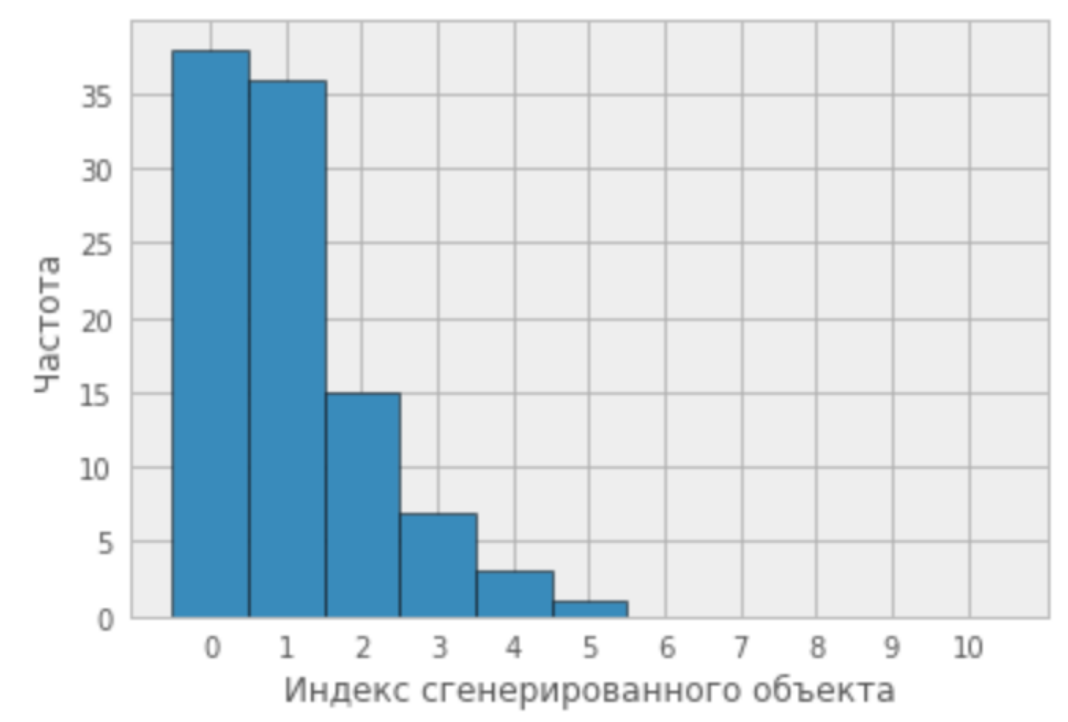
\includegraphics[width=0.7\linewidth]{Dissertation/pics/geom_distr_2}
    \caption{Зависимость количества объектов от сгенерированного индекса}
  \end{minipage}
  \label{img:geom_distr_2}
\end{figure}
После того, как положительные примеры обучающей выборки собраны, необходимо создать также и отрицательные примеры. Для отрицательных примеров используется следующий алгоритм:
\begin{enumerate}
    \item построение графа ключевых слов $\hat{G}$ по модифицированному множеству ключевых слов;
    \item для каждого слова $w$, попавшего в множество пар положительных примеров, рассматриваются случайные $k$ соседей $v_1, v_2, ..., v_k$ на расстоянии $2$ в графе $\hat{G}$;
    \item все пары $(w, v_i)_{i=1}^k$ принимаются отрицательными примерами.
\end{enumerate}

Мотивация данного алгоритма в следующем. Для обучения модели отрицательные примеры должны быть содержательными: если рассматреть случайные пары ключевых слов без каких-либо дополнительных условий, то большинство полученных примеров не будут представлять особой значимости для модели, потому что большинство статистических характеристик будут нулевыми или слишком малыми (между случайными вершинами в графе может не быть путей, они могут не иметь общих соседей, могут быть расположены на слишком большом удалении друг от друга и т.д.). Очень вероятно, что такие абсолютно случайные пары действительно не имеют и модель действительно легко научится различать положительные и отрицательные экземпляры выборки. Однако,  это не дает никакой информации для модели для более сложных случаев, когда слова находятся достаточно близко друг к другу в графе и имеют достаточну большую вероятность быть похожими. И именно такие случаи и представляют интерес в рамках данной задачи.

С другой стороны, если для вершины в качестве отрицательных примеров брать непосредственных соседей в графе (то есть максимально близкие вершины), то слишком часто будут появляться пары, которые в действительности близки по смыслу. Это происходит потому, что среди слов одного набора могут встречаться похожие слова. В следствии этого, среди отрицательных примеров будет большое число false-negative примеров (то есть примеров, которые ошибочно были промаркированы отрицательными), что не позволит качественно обучить модель.

Поэтому соседи вершины на расстоянии $2$ видятся наиболее подходящим компромиссом: среди них не так часто встречаются семантически близкие пары, но при этом они несут в себе содержательный сигнал, на котором можно эффективно обучаться.
\subsubsection{Окончательная версия алгоритма}

\begin{itemize}
    \item Входные параметры: $N$, $p$, $k$;
    \item для каждого набора ключевых слов $W \in W_X$ системы $X$:
        \begin{itemize}
            \item для каждого \textit{вхождения} ключевого слова $w$:
                \begin{itemize}
                    \item если количество вхождений в коллекцию превосходит пороговое значение $N$:
                        \begin{itemize}
                            \item из геометрического распределения с параметром $p$ выбирается число;
                            \item вхождение ключевого слова $w$ заменяется $w@p$;
                            \item слово $w@p$ заносится в список модификация для слова $w$;
                        \end{itemize}
                    \item иначе
                        \begin{itemize}
                            \item вхождение ключевого слова $w$ заменяется $w@0$;
                        \end{itemize}
                \end{itemize}
            \item модифицированная версия набора ключевых слов добавляется в множество $W^{*}_X$
        \end{itemize}
    \item для каждого уникального ключевого слова $w$
        \begin{itemize}
            \item каждую пару модификаций $(w@i, w@j)$ ключевого слова $w$ добавить в обучающее множество $X_{train}$ в качестве положительного примера;
        \end{itemize}
    \item для модифицированной версии коллекции наборов ключевых слов $W^{*}_X$ добавить произвести построение графа ключевых слов $G^{*}$;
    \item для каждой вершины $w@i$ из множества модифицированных вершин графа $G^{*}$:
        \begin{itemize}
            \item выделить множество  $G_{2}(w@i) = neigbors(G^{*}, w@i, 2)$ соседей вершины $w@i$ в графе $G^{*}$ на расстоянии $2$
            \item из множества $G_{2}(w@i)$ выбрать случайно $k$ вершин $v_1, ... v_k$ и для каждой вершины добавить пару $(w@i, v_j)$ в $X_{train}$ в качестве отрицательного примера.
        \end{itemize}
\end{itemize}

Значения параметров $N$, $p$, $k$ были определены как $10$, $0.9$, $5$ соответственно.

Вхождением ключевого слова в описанном выше алгоритме является появление ключевого слова в одном конкретном наборе ключевых слов. Поскольку одно слово может присутствовать во многих наборах, то число вхождений равно количеству наборов, содержащих данное ключевое слово.


\textbf{Утверждение 3.} Расчет искусственной обучающей выборки имеет сложность $O(f^2 * k + w^2 * k^2)$, где $f$ - максимальная частотность слова в коллекции, $k$ - количество уникальных слов в коллекции, $w$ - максимальный размер набора в коллекции ключевых слов.

%Процедура $m$ - максималь
%кол-во уникальных k
%кол-во наборов m
%максимальное число слов в наборе w
%максимальная частотность слова в коллекции f
%w * m - прошли по наборам, модиф кл слова.
%
%f * k - все наборы, один раз прошлись
%f^2 - модификаций для одного слова
%f^2 * k - для всех
%f * k - построение графа
%k - максимальный размер набора (все уникальные слова попали в один набор)
%k * k  (http://www.cs.tau.ac.il/~zwick/papers/sparse.pdf умножение matr n*n -> m*n , m=nnz)
% http://www.stat.ucdavis.edu/~chohsieh/teaching/ECS289G_Fall2015/complexity.pdf
%f^2 * k + k^2

\textbf{Лемма 1.} Расчет положительных примеров искусственной обучающей выборки имеет сложность $O(f^2 * k)$, где $f$ - максимальная частотность слова в коллекции, $k$ - количество уникальных слов в коллекции.

\textbf{Доказательство.} 
Число всех ключевых слов системы с повторениями не превышает значение $f * k$. Необходимо пройти один раз по всем ключевым словам коллекции, чтобы сгенерировать для них модифицированную версию - это требует $O(f * k)$ времени. При этом полагается, что выбор случайного числа из выбранного распределения занимает константное время. Следующим шагом необходимо из модифицированных версий каждого слова получить всевозможные пары. Для каждого из $k$ слов может быть получено не более, чем $f$ модификаций слова, поскольку каждая модификация была получена из некоторого исходного слова, которое в свою очередь было использовано не более, чем $f$ раз в коллекции. Для генерации всех пар для данного исходного слова необходимо $O(f^2)$ времени, а для всех уникальных слов - $O(k * f^2)$.

\textbf{Лемма 2.} Расчет отрицательных примеров искусственной обучающей выборки имеет сложность $O(w^2 * k^2)$, $k$ - количество уникальных слов в коллекции, $w$ - максимальный размер набора в коллекции ключевых слов.

\textbf{Доказательство.} 
. Построение графа ключевых слов занимает не более $O(k^2)$ времени. Далее необходимо рассчитать соседей для каждой вершины на расстоянии $2$. Для этого необходимо возвести в квадрат матрицу смежности графа. При хранении графа в виде разреженной матрицы, операция умножения матрицы размера $(k*k)$ на себя требует $O(nnz * k)$ операций, где $nnz$ - количество ненулевых элементов. Поскольку в графе ключевых слов ребрами являются те пары ключевых слов, которые входят в один набор, то количество ребер в графе, как и количество ненулевых элементов в матрице смежности, не превышает $O(w^2 * k)$, то сложность поиска соседей второго порядка будет равна $O(w^2 * k^2)$. Предполагая, что операция взятия случайного числа занимает константное время, получаем, что генерация отрицательных примеров для искусственной обучающей выборке требует $O(w^2 * k^2)$ операций.

Из двух доказанных выше лемм немедленно следует утверждение 3.

%\begin{Алгоритмо
\subsection{Признаковое описание модели машинного обучения} \label{sec:features}
Под признаковым описанием пары ключевых слов понимается определение набора функций, вычисляющих некоторые числовые характеристики для рассматриваемых слов. Такие функции (факторы) могут использовать оба слова в явном виде (расстояние Левенштейна, количество общих слов и т.д.) или только одно из слов (частотность данного слова в корпусе, количество символов в слове и т.д.), что порождает пару значений признака для левого и правого слов из пары. Благодаря древовидной структуре решающих алгоритмов подсчитанные факторы не обязаны коррелировать с целевой переменной, чтобы улучшать качество классификации. 

Таким образом, в ходе работы алгоритма для всех рассматриваемых пар ключевых слов происходит вычисление всего набора факторов, что образует матрицу объект-признак, строка которой является описанием конкретной пары ключевых слов, а столбец определяет значения некоторого признака для все пар. Для обучающей выборки помимо матрицы объект-признак также имеется вектор-столбец истинных значений. Это позволяет обучать алгоритмы машинного обучения, после чего применять обученные модели для предсказания на новых данных (для которых также получить признакое описание). 



%\begin{tabularx}{10cm}{|p{4cm}|p{4cm}|p{2cm}|}
\begin{tabularx}{16cm}{|X|X|X|}
        \hline
        Признак & Описание & Тип \\ \hline
        Расстояние в графе ключевых слов & & Парный \\ \hline
        Расстояние в усеченном контекстном графе ключевых слов & & Парный/графовый \\ \hline
        Контекстная близость & Вариации контекстной близости, описанные в подразделе \ref{cont_sim} & Парный/графовый \\ \hline
        Ранк контекстной близости & & Парный/графовый \\ \hline
        Мера абстрактности & Мера общности понятия, описанная в разделе \ref{abstract_words_chapter} & Одиночный/графовый \\ \hline
        Количество вершин в кластере & Количество вершин описанного в \ref{clustering_section} кластера для рассматриваемой вершины & Одиночный/графовый \\ \hline
        PageRank вершины графа & Значение PageRank меры для вершин графов & Одиночный/графовый \\ \hline
        EdgeRank ребра графа & Значение EdgeRank меры для ребер графов & Парный/графовый \\ \hline
        Вес ребра в графе ключевых слов & & Парный/графовый \\ \hline
        Частотность левого слова & & Одиночный/графовый \\ \hline
        Частотность правого слова & & Одиночный/графовый \\ \hline
        Совместная частотность в корпусе & & Парный/графовый \\ \hline
        Pointwise mutual information & & Парный/графовый \\ \hline
        Мера Жаккара & Считается по вершинам соседям & Парный/графовый \\ \hline
        Число простых путей в графах между вершинами & Считается по обоим графам & Парный/графовый \\ \hline
        Betweenness centrality  & & Одиночный/графовый \\ \hline
        Closeness centrality & & Одиночный/графовый \\ \hline
        Eigen vector centrality & & Одиночный/графовый \\ \hline
        Значение потока между вершинами & & Парный/графовый \\ \hline
        Количество соседей & На расстоянии 1 и 2 (два фактора) & Одиночный/графовый \\ \hline
        Количество общих соседей & На расстоянии 1 и 2 (два фактора) & Парный/графовый \\ \hline
        Расстояние Левенштейна & & Парный/языковой \\ \hline
        Часть речи слова & Категориальный признак & Одиночный/языковой \\ \hline
        Количество слов  & & Одиночный/языковой \\ \hline
        Количество букв & & Одиночный/языковой \\ \hline
        Количество общих слов & & Парный/языковой \\ \hline
        Пословная мера Жаккара & & Парный/языковой \\ \hline
        Нграммная мера Жаккара & Используется биграмное и триграмное представление слов & Парный/языковой \\ \hline
        Пара слов на разных языках & Бинарный признак & Парный/языковой \\ \hline
        Одно слово является аббревиатурой/сокращением  для другого & Бинарный признак & Парный/языковой \\ \hline
        Одно слово является формой другого & Бинарный признак & Парный/языковой \\ \hline
        Одно слово является транслитерацией другого & Бинарный признак, использован наивный алгоритм транслитерации & Парный/языковой \\ \hline
        Расстояние по дереву WordNet & & Парный/языковой \\ \hline
        Глубина слова в дереве WordNet & & Одиночный/языковой \\ \hline
        Косинусное расстояние между word2vec представлениями слов & & Парный/языковой \\ \hline
        Средняя частотность слов в корпусе & В качестве слов рассматриваются не ключевые слова, а отдельные слова естественного языка  & Одиночный/языковой \\ \hline
        Косинусное расстояние пословных TFIDF представлений & В качестве слов рассматриваются не ключевые слова, а отдельные слова естественного языка & Парный/языковой \\ \hline
        Косинусное расстояние нграммных TFIDF представлений & Подсчитано на символьных триграммах & Парный/языковой \\ \hline

\end{tabularx}

В таблице \ref{tbl:features} представлен набор факторов, который был использован в работе для обучения модели. Графовыми факторами являются те факторы, которые возможно посчитать по графам, описанным в предыдущих главах. Графовые признаки ни в каком виде не учитывают содержимое вершин графа, т.е. абстрагируются от описания ключевого слова на естественном языке и используют только его связи с другими вершинами в рассматриваемом корпусе данных. Языковые признаки, напротив, используют знания из области обработки естественного языка: морфологические, синтаксические и семантические.

\subsection{Описание и настройка модели машинного обучения} \label{sec:model}
Основную идею можно описать следующим образом. Для решения задачи выбирается множество пар ключевых слов, которые являются близкими по смыслу, а также множество пар, которые напротив, далеки друг от друга по смыслу. Эти два множества вместе составляют обучающую выборку или разметку. Способы получения обучающих выборок были описаны в предыдущих разделах. Следующим шагом выбирается метрика (т.н. функция потерь), которую алгоритм будет оптимизировать в ходе обучения. К данной задаче применительны как функции потерь для задач классификации (например, логарифмическая функция потерь), так и функции потерь для задач регрессии (такие как среднеквадратичная ошибка). Несмотря на то, что первое семейство метрик более естественно для решаемой  задачи (поскольку решается задача бинарной классификации: является ли пара ключевых слов близкой по смыслу или нет), по результатом экспериментов, рассмотрение задачи определения семантической близости как задачи регрессии может даже более качественный результат. Далее выбирается алгоритм машинного обучения, на вход которому подается признаковое описание элементов обучающей выборки, а также истинные ответы для объектов этой обучающей выборки. Множество признаков детально описано в разделе \ref{sec:features}. В рамках рассматриваемой задачи наилучшее качество продемонстрировала реализация алгоритма градиентного бустинга на решающих деревьях XGBoost. Отмечается, что обучение алгоритмов также непрерывно связано с настройкой гиперпараметров, но в данном случае это значительно более простая задача, поскольку для конкретного алгоритма машинного обучения есть набор рекомендаций по настройке параметров. Также существует программные комплексы, способные настроить гиперпараметры в автоматическом режиме. После того, как модель обучена, можно применять её к произвольным парам ключевых слов, предварительно посчитав для них их признаковое описание. На выходе будет степень уверенности модели в том, что пара слов является семантически похожими понятиями.



\section{Построение тезауруса ключевых слов по коллекции наборов} \label{thes}

\begin{figure}[ht]
  \begin{minipage}[ht]{1.0\linewidth}\centering
    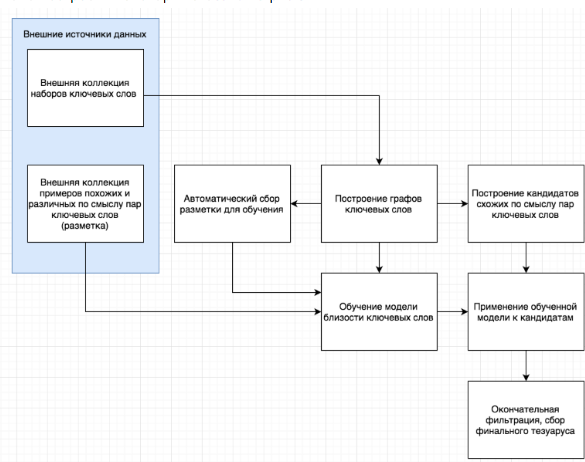
\includegraphics[width=0.7\linewidth]{Dissertation/pics/thes}
    \caption{Схема построения словаря тезауруса ключевых слов}
  \end{minipage}
  \label{img:thes}
\end{figure}

В качестве внешних данных используется коллекция наборов ключевых слов научных публикаций, собранная из сети Веб. Это коллекция, насчитывающая сотни тысяч наборов ключевых слов для русскоязычных статей и миллиона наборов на английском языке. С помощью этих наборов поочередно строится несколько графов близости. Одним из таких графов является, например, граф, в вершинах которого находятся ключевые слова, а в ребро означает причастность двух ключевых слов одному набору. Вес ребра тем больше, чем чаще пара слов встречается в одном наборе. Другим примером контекстного семантического графа является граф, в вершинах которого как и прежде стоят ключевые слова, а ребра указывают на наличие у этой пары общего ключевого слова, которое входит в некоторые наборы вместе и с первым словом из пары, и со вторым (но не с двумя сразу). Было показано, что ребра такого графа гораздо сильнее отражают семантическую близость, в то время как ребра первого графа служат для улучшения механизмов поисковых подсказок, потому что предлагают связанные, но более разнообразные слова для заданного.

Также внешними данными является коллекция достоверно похожих и различных пар ключевых слов (разметка). Такая разметка необходима для настройки алгоритмов и тестирования качества их программных реализаций. В эту разметку входят открытые базы синонимов, антонимов, аббревиатур, а также некоторые переводы на другие языки.

Помимо словарной разметки, при построении тезауруса на базе графов ключевых слов генерируется автоматическая разметка. Преимущество этой разметки в том, что она полностью строится по данным, что означает отсуствие необходимости иметь внешнюю собранную вручную разметку (обычно это дорогой и трудоемкий процесс). Вместе с этим, автоматическая разметка не вносит смещение в данные. Например, если в базах синонимов встречается много математических терминов, но мало биологических, то модель настроится на то, чтобы давать парам математических терминов большее значение близости. 

В то же время автоматическая разметка будет использовать обучающие примеры из разных областей ровно в той пропорции, в которой они представлены в конкретных данных. С другой стороны, такая разметка может быть менее точной, поэтому в финальной версии алгоритма используется обе разметки.

Поскольку ключевых слов достаточно много, то рассмотреть все пары не представляется возможным, поэтому по построенным графам строятся кандидаты близких по смыслу пар ключевых слов. Их количество достаточно велико, но значительно меньше всех возможных пар.

После этого для пар-кандидатов подсчитываются числовые факторы: различные расстояния и характеристики в графе, статистические показатели и другие. По этим факторам строится модель, которая настраивается с помощью разметок, описанных выше. Затем модель применяется к парам-кандидатам и те пары, которым модель дала наибольший вес, проходят в окончательный словарь ключевых слов.

\subsection{Тестовые испытания}
Далее приводятся результаты тестирования программных реализаций описанных алгоритмов определения близости. Рассмотрены два способа проведения тестовых испытаний: на отложенной части обучающей выборки и на множестве пар одинаковых слов.

\subsubsection{Тестирование на отложенной выборке}
Тестирование программных реализаций алгоритмов проводилось по следующему сценарию. Из обучающей выборки, собранной с помощью эвристических методов была выделена тестовая часть, которая не принимала участия в обучении моделей. После этого обучалось несколько моделей:
\begin{itemize}
    \item модель, обученная на эвристической обучающей выборке с использованием языковых признаков;
    \item модель, обученная на эвристической обучающей выборке с использованием графовых признаков;
    \item модель, обученная на эвристической обучающей выборке с использованием языковых и графовых признаков;
    \item модель, обученная на искусственной обучающей выборке с использованием графовых признаков;
    \item модель, обученная на эвристической и искусственной обучающих выборках с использованием графовых признаков;
\end{itemize}

Далее качество тестировалось на тестовой части обучающей выборки. Результаты приведены в таблице \ref{tbl:sim_res}

\begin{tabularx}{16cm}{|X|X|X|}
        %\label{tbl:sim_res}
        \hline
        Обучающее множество & Набор факторов & Значение F-меры \\ \hline
        Эвристическое & Языковые & 0.85 \\ \hline
        Эвристическое & Графовые & 0.75 \\ \hline
        Эвристическое и искуственное & Графовые & 0.81 \\ \hline
        Искусственное & Графовые & 0.79 \\ \hline 
        Эвристическое & Графовые и языковые & 0.88 \\ \hline
        - & Word2Vec & 0.69 \\ \hline 
\end{tabularx}

\subsubsection{Тестирование тождественно равных пар} \label{sec:test_equal}
Суть эксперимента в следующем: очевидно, что самым ближайшим по смыслу словом является оно само. Поэтому необходимо, что модель могла определять, что для слова $w$ среди всех возможных кандидатов, самым ближайшим по смыслу будет само слово $w$. В разработанную модель явным образом не закладывается информация о таком свойстве метрики, поскольку среди обучающих примеров не было таких пар, в которых слова не отличались. Это делает эксперимент осмысленным и дает представление об адекватности разработанной модели.

Для каждого из $10000$ случайных ключевых слов были подсчитаны меры близости для $1000$ других случайных слов (в том числе близость и до рассматриваемого слова). В более, чем $99.9\%$ случаев наиболее близким для рассматриваемого слово было определено оно само же. Таким образом, модель с большей уверенностью можно считать качественной.


\section{Выводы}

По результатам тестовых испытаний программных реализаций можно заключить, что разработанные графовые алгоритмы улучшают качество определения семантических связей между объектами. Алгоритмы, реализации которых были использованы в качестве факторов для модели предсказания степени близости, увеличивают значение F-меры на тестовой выборке, а следовательно, являются полезными. 

Помимо этого отмечается, что благодаря алгоритму искусственной генерации обучающей выборки, появляется возможно получить качественную модель, несмотря на отсутствие настоящих примеров для обучения. Было показано, что такая модель не сильно уступает по качеству модели, обученной на реальных примерах, сбор которых является ресурсозатратным.

